\chapter{Simulations}\label{chap:Simulations}

\section{Introduction}

In this chapter, we carried-out simulations with synthetic patient arrival datasets and compares the posterior distribution results and prediction rate between Independent Bayes Model (IBM) and Hierarchical Bayes Model (HBM) in scenarios of with different anomalies and different hierarchy structures. Sections 2.1 details functions used to synthesis simulation datasets. Sections 2.2 evaluate the use of different priors for Bayesian Models to used during the simulations. Section 2.3 explores the impact of the size of the anomaly on anomaly detection at different levels of hierarchy. Lastly, section 2.4 considers how the complexity of the hierarchical structure affects anomaly detection at different levels of hierarchy. 
%add \ref{} to sections

\section{Simulation Methods}

All datasets used for the simulation studies are synthetically generated. Synthetic datasets refer to data information artificially manufactured rather than generated from real-world events. Synthetic data takes preference over the alternative option, perturbed data, a dataset generated by adding alteration and noise to real-world data \citep{drechsler2008comparing, drechsler2011synthetic}. Advantages of synthetic data include (1) Disclosure protection, making sure no sensitive information about individuals from the public can not be leaked or extracted. (2) Reduce the effects of possible background noises presented in real-world data. (3) Allows control over the hierarchical structure of datasets, note that real-world hierarchical data are often extremely complex and can have lots of levels, and complexity that comes with it, increasing the difficulty to control our simulations, and making interpretations difficult.  


\newpara

Several custom R-functions has been created to synthesis datasets used in our studies,  Appendix~\ref{Rfun} provides descriptions of the custom functions. There are several reasons for creating custom simulation synthesis functions. Firstly, a large number of simulated datasets with variable settings were expected to be required to perform our analyses; this required a large number of custom function arguments that existing packages may not contain. Secondly, synthetic datasets were simulated to mimic a health dataset in a purely theoretical setting. Thirdly, an emphasis was placed on the hierarchical nature of particular variable of the dataset (for example, ICD codes and geographic location), custom structure hierarchical structures can be used to generate branching, and nodes during the simulation process. Lastly, for exploration research, it was unclear what functionalities were needed, existing statistical data simulation packages may become insufficient at a later stage.

\begin{figure}[!t]
	\centering
	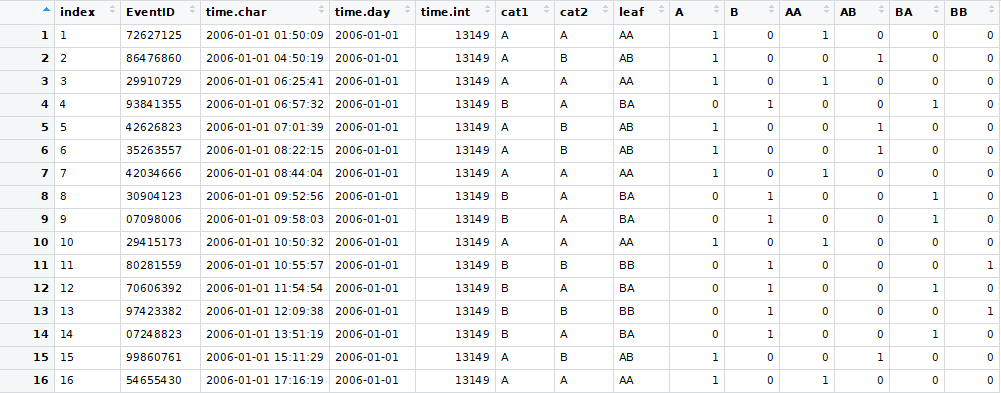
\includegraphics[width=1.0\linewidth]{Figures/rawdata}
	\caption{Entries of the raw dataset}
	\label{fig:rawdata}
\end{figure}

\newpara

\texttt{simdata} and \texttt{adddaily.anomaly} are the two major function used during the data synthesis process. \texttt{simdata} function were used to synthesise a raw dataset (figure~\ref{fig:rawdata}) that simulate a hospital record that you would typically found in hospital digital archives, where each row corresponds to a single entry of hospital event with a unique hospital event identifier. The function automatically generates Time, dates and various information about the hierarchical structure. The default number of simulation is 1,000,000, and default period is a 12 year-long period between 1 January 2006 and 31 December 2018, and a matrix that contains information of the hierarchical structure are manipulated and used to produce a hierarchical structure with different characteristics.

\newpara

The matrix used in the argument of \texttt{simdata} function contains the theoretical value of each leaf of a two-level hierarchical structure in a proportion out of 1000. This matrix is used to specify the hierarchical structure for each of our simulated data. As shown with the simplified example in  figure~\ref{fig:flow}, for example, if the theoretical value at of the leaves (refers to categories at the very bottom level hierarchy) are 8, 8, 5, and 3, the function will convert and  represent this information with a matrix with standard numbers 333,333,209 and 125. Each column corresponds to a single group; therefore, column sums of the matrix correspond to the count of a level 1 categories, and the sum of all numbers in the matrix equal to the total count. The parent levels are simply the sum of children levels, and the complete hierarchical structure can be generated automatically just from numerical information of leaves. Note that the number of column of the matrix corresponds to the maximum number of leaves within a level 1 category, for level 1 categories with less than maximum amount of leaves, 0 is used to represent no leaf. The default value of the matrix is 250, 250, 250 and 250, which represent a two-level hierarchical of equal proportions, with 2 level-1 categories, each with 2 level-1 categories of equal proportions.Note the function can be used to generate all possibilities of 2-level hierarchical model, not just the 4 leaf example that is shown here, the use of out of 1000 (instead of being four non-negative real numbers which add to 1, which makes better sense) is a personal choice because it makes coding easier. This way of storing hierarchical information is simple and efficient but is not suitable for hierarchical models that contain 3 or more levels, and maybe a little confusing for other people at first, future improvements of the function could be allowing usage of a user-generated hierarchical time series (\texttt{hts}) object from the \texttt{hts} package instead of the matrix, to allow generations of  hierarchical dataset with  3 or more levels. 

\newpara 

\begin{figure}[!t]
	\begin{equation*}
	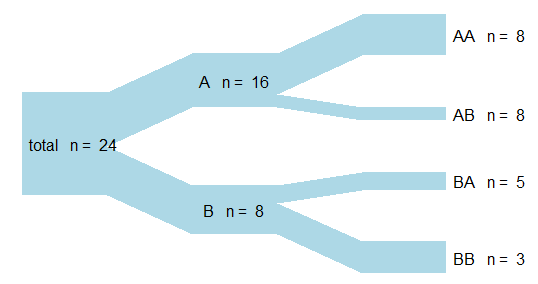
\includegraphics[width=0.7\linewidth]{Figures/flow1} 
	\Rightarrow
	\begin{bmatrix}
	8 & 5 \\
	8 & 3 \\
	\end{bmatrix}
	\Rightarrow
	\begin{bmatrix}
	333 & 208 \\
	333 & 125 \\
	\end{bmatrix}
	\end{equation*}
	\caption{Conversion of a simple hierarchical structure to a matrix}
	\label{fig:flow}
\end{figure}

\begin{figure}[!h]
	\centering
	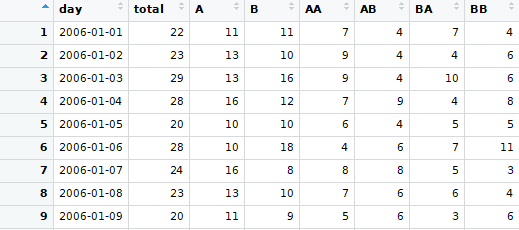
\includegraphics[width=0.7\linewidth]{Figures/dailydata}
	\caption{Entries of the daily count dataset}
	\label{fig:dailydata}
\end{figure}


\texttt{adddaily.anomaly} were used to \texttt{addanomaly} function to add anomaly to daily count data(number of hospital arrivals), a hierarchical time-series dataset generated by tabulating the raw synthesised dataset (with each entry representing a hospital arrival event)using \texttt{tabulatedata} function. The default setting for anomaly is a point anomaly of 1 day, on 2015-11-15. The amount of anomaly added are in terms of the proportion of the total count (For example, a 25\% anomaly here meant an addition of 25\% of the count of category total, on top of the hierarchy,in mathematical terms $1.25y_{total,t}$, in other words, if we expect 100 hospital arrival events, an arrival rate of 125 meant a 25\% anomaly has occurred), and amount of anomaly assigned to each leaf (subcategories, in this thesis, different ICD codes) can be varied. This controls the size of overall anomaly and allows for customisation of hierarchical structure at lower levels, the plan is to give the freedom to explore how different hierarchical structure would affect the results of our hierarchical and independent models. 


\newpara

For point anomalies the amount of anomaly assigned to each leaf is transcribed with binding of 3 vector: (1) a vector of amount of anomaly to be added to total,  (2) a vector of amount of anomaly to be added to level 1 categories and (3) a vector of amount of anomaly to be added to level 2 categories, all in values of proportions. In mathematical thinking, we could think of binding as additions of $n*m$ matrices, where information only exist on certain row or columns, and addition of the column or rows condense all the information together.  For example, for a hierarchical time series with the same hierarchical structure as the example given in figure \ref{fig:flow}, if we want to add all of our anomalies to AA, the proportion vector of anomaly for total is $\{1\}$ and this will be the case for any hierarchical structure because the proportion of all categories will sum to 1. The proportion vector of anomaly for level 1 categories is $\{1,0\}$ and the percentage vector for level 2 categories is $\{1,0,0,0\}$, so the proportion vector that is required for our function to indicate our setup, is $\{1,1,0,1,0,0,0\}$. 

\begin{figure}[!h]
	\begin{equation*}
	\begin{aligned}
	P_{total} \quad 
	P_{lv1} \quad \quad \quad \quad  
	P_{lv2} \quad \quad \quad & 
	\quad \quad \quad  \quad \quad  P \\
	\begin{bmatrix}
	1 \\
	\end{bmatrix}
	+
	\begin{bmatrix}
	1 & 0\\
	\end{bmatrix}
	+
	\begin{bmatrix}
	1 & 0 & 0 & 0\\
	\end{bmatrix}
	\Rightarrow &
	\begin{bmatrix}
	1 & 1 & 0 & 1 & 0 & 0 & 0\\
	\end{bmatrix}
	\end{aligned}
	\end{equation*}
	\caption{Construction of the proportion vector}
	\label{fig:vec}
\end{figure}

In summaries, \texttt{simdata} and several supporting functions were used to generate simulated data, and then we manually added different anomalies with \texttt{adddaily.anomaly} function. The whole process resulted in 60 various simulated datasets with same default setting (refer to details on \texttt{simdata}), different hierarchical structure and different added anomalies that are used for this section. 

\newpara

Details about setups used for the data synthesis process can be found in the start of each section of our simulation tests, and the R codes used can be found in \texttt{91-createdata-test.R}, \texttt{92-createdata-anoamly.R}, \texttt{93-createdata-proportion.R} and \texttt{94-createdata-count.R} found in GitHub Repository: \href{https://github.com/jungxue/research-masters-Jung}{https://github.com/jungxue/ research-masters-Jung}. 

%------------------------------------------------------------------------------------------        
\newpage

\section{Simulation 1: Prior}

\subsection{Priors}

For Bayesian inference to make sense, a prior is essential and often required. However, there are different ways in which prior can be generated. For simulations, no external information is available; therefore, the informative prior approach is out of the question. However, it is possible for us to assign relatively simple weak-informative and non-informative priors by generating probability distributions with vaguely defined parameters. Hence, we proposed six different priors that express different hypothesised information about the prior and test how they affect our posterior distribution calculations. 
\newpara

A simple Poisson process can be used to model for a random, and mutually independent arrivals rate, with the likelihood model:

\begin{equation*} \label{Poisson}
\begin{aligned}
y_{,t} & \sim Poisson(\mu_{i,t}) \\  
log(\mu_{i,t}) & = log(\rho_{i,t}) \\
\end{aligned}
\end{equation*}

For the Poisson process, observations $y_{i,t}$ ($y$ of $i$th category given time $t$) is hypothesised to follow the distribution of the Poisson process, with parameter $\mu_{i,t}$ stand for the expected number of arrivals per time-interval(In this study we are actually only looking at one particular day/time interval, so t actually does not vary, but the notation is still included to make general sense) And $\rho_{i,t}$ as the log equivalent. For our simulations, this time interval is set up to be a 12 year-long period between 1 January 2006 and 31 December 2018.The sum of simulated arrival entries sum to 1,000,000. Distributions of priors can then assigned to $\mu_{i,t}$, this provides essential information to the parameter and will have a significant impact in our calculations. Samples of the JAG codes used to build our models is presented in appendix~\ref{models}, and complete JAGS codes and R codes used to obtain our graphical results are available on GitHub repository:
\href{https://github.com/jungxue/research-masters-Jung}{https://github.com/jungxue/research-masters-Jung}. 

\subsubsection{Model 1 Non-informative Prior}

Model 1 is an Independent Bayesian Model with no priors that models each categories independently on all hierarchical levels. This model provides no information for the estimation of distribution parameter $\mu_{i,t}$, and therefore the prior can be defined as a non-informative prior (although this term often refers to flat prior), here in this thesis we call it the null prior. The likelihood model for Poisson model with null prior is:

\begin{equation*} \label{Poissonm1}
\begin{aligned}
y_{i,t} & \sim Poisson(\mu_{i,t}) \\  
log(\mu_{i,t}) & = log(\rho_{i,t}) \\
\end{aligned}
\end{equation*}

\subsubsection{Model 2 Normal($\mu$=1,$\sigma^-2$=0.3) Prior}

Model 2 is an Independent Bayesian Model with $\rho \sim Normal(1, 0.3)$ prior that models each categories independently on all hierarchical levels. This model does contain information for the estimation of distribution parameter $\mu_{i,t}$, and therefore the prior can be defined as a weak-informative prior. $I_{[\lambda>0]}$ indicates truncation of distribution at 0; in other words, the prior does not contain$\lambda_{i,t}$ with values less than 0 and should not contain any negative values. The likelihood model for a Poisson process with a $Normal(1, 0.3)$ prior is:

\begin{equation*} \label{Poissonm2a}
\begin{aligned}
y_{i,t} & \sim Poisson(\mu_{i,t}) \\  
log(\mu_{i,t}) & = log(\rho_{i,t}\lambda_{i,t}) \\
\end{aligned}
\end{equation*}

Priors for model parameters:

\begin{equation*} \label{Poissonm2b}
\begin{aligned}
\lambda_{i,t} & \sim Normal(\mu_{i,t},\sigma_{i,t}) I_{[\lambda>0]}\\
\end{aligned}
\end{equation*}

Hyper-priors for model parameters:

\begin{equation*} \label{Poissonm2c}
\begin{aligned}
\mu_{i,t} & \sim Normal(1,0.1)\\
\sigma^2_{i,t} &\sim Normal(0.3,0.1)\\
\end{aligned}
\end{equation*}

\subsubsection{Model 3 Normal($\mu$=1,$\sigma^-2$=0.1) Prior}

Model 3 is an Independent Bayesian Model with $\rho \sim Normal(1, 0.1)$ priors that models each categories independently on all hierarchical levels. This model does contain information for the estimation of distribution parameter $\mu_{i,t}$, and therefore the prior can be defined as a weak-informative prior. $I_{[\lambda>0]}$ indicates truncation of distribution at 0; in other words, the prior does not contain$\lambda_{i,t}$ with values less than 0 and should not contain any negative values. The likelihood for a Poisson process with a $Normal(1, 0.1)$ prior model is:

\begin{equation*} \label{Poissonm3a}
\begin{aligned}
y_{i,t} & \sim Poisson(\mu_{i,t}) \\  
log(\mu_{i,t}) & = log(\rho_{i,t}\lambda_{i,t}) \\
\end{aligned}
\end{equation*}

Priors for model parameters:

\begin{equation*} \label{Poissonm3b}
\begin{aligned}
\lambda_{i,t} & \sim Normal(\mu_{i,t},\sigma_{i,t}) I_{[\lambda>0]}\\
\end{aligned}
\end{equation*}

Hyper-priors for model parameters:

\begin{equation*} \label{Poissonm3c}
\begin{aligned}
\mu_{i,t} & \sim Normal(1,0.1)\\
\sigma^2_{i,t} &\sim Normal(0.1,0.1)\\
\end{aligned}
\end{equation*}

\subsubsection{Model 4 Gamma($alpha$=4,$beta$=3) Prior}

Model 4 is an Independent Bayesian Model with $\rho \sim Gamma(4, 3)$ priors that models each categories independently on all hierarchical levels. This model does contain information for the estimation of distribution parameter $\mu_{i,t}$, and therefore the prior can be defined as a weak-informative prior. $I_{[\lambda>0]}$ indicates truncation of distribution at 0; in other words, the prior does not contain$\lambda_{i,t}$ with values less than 0 and should not contain any negative values. The likelihood model for Poisson process with  $Gamma(4, 3)$ prior is:

\begin{equation*} \label{Poissonm4a}
\begin{aligned}
y_{i,t} & \sim Poisson(\mu_{i,t}) \\  
log(\mu_{i,t}) & = log(\rho_{i,t}\lambda_{i,t}) \\
\end{aligned}
\end{equation*}

Priors for model parameters:

\begin{equation*} \label{Poissonm4b}
\begin{aligned}
\lambda_{i,t} & \sim Gamma(\alpha_{i,t},\beta_{i,t}) I_{[\lambda>0]}\\
\end{aligned}
\end{equation*}

Hyper-priors for model parameters:

\begin{equation*} \label{Poissonm4c}
\begin{aligned}
\alpha_{i,t} & \sim Normal(4,0.1)\\
\beta_{i,t} &\sim Normal(3,0.1)\\
\end{aligned}
\end{equation*}

\subsubsection{Model 5 Laplace($alpha$=1,$beta$=1) Prior}

Model 5 is an Independent Bayesian Model with $\rho \sim Laplace(1, 1)$ priors that models each categories independently on all hierarchical levels. This model does contain information for the estimation of distribution parameter $\mu_{i,t}$, and therefore the prior can be defined as a weak-informative prior. $I_{[\lambda>0]}$ indicates truncation of distribution at 0; in other words, the prior does not contain$\lambda_{i,t}$ with values less than 0 and should not contain any negative values. The likelihood model for Poisson process with $Laplace(1, 1)$ prior is:

\begin{equation*} \label{Poissonm5a}
\begin{aligned}
y_{i,t} & \sim Poisson(\mu_{i,t}) \\  
log(\mu_{i,t}) & = log(\rho_{i,t}\lambda_{i,t}) \\
\end{aligned}
\end{equation*}

Priors for model parameters:

\begin{equation*} \label{Poissonm5b}
\begin{aligned}
\lambda_{i,t} & \sim Laplace(\alpha_{i,t},\beta_{i,t}) T_{[\lambda>0]}\\
\end{aligned}
\end{equation*}

Hyper-priors for model parameters:

\begin{equation*} \label{Poissonm5c}
\begin{aligned}
\alpha_{i,t} & \sim Normal(4,0.1)\\
\beta_{i,t} &\sim Normal(3,0.1)\\
\end{aligned}
\end{equation*}

\subsubsection{Model 6 Mixture Prior}

Lastly, Model 6 is an Independent Bayesian Model with a mixture prior that models each category independently on all hierarchical levels. The prior is thought to be a mixture of no information and weak information, in other words, we are proposing that for most of the time there is no variation, and for some of the time, there is information. The idea comes from \citet{berry2004}, where they proposed a scenario where the majority of the difference between treatment and control is zero, and there are just some variations. However note that their prior is an one-sided distribution that centre at 0, and our prior is two-sided and centre at 1. This model does contain information for the estimation of distribution parameter $\mu_{i,t}$, and therefore, the prior can be defined as a weak-informative prior. $I_{[\lambda>0]}$ indicates truncation of distribution at 0; in other words, the prior does not contain$\lambda_{i,t}$ with values less than 0 and should not contain any negative values. The likelihood model for a Poisson model process with mixture prior is:

\begin{equation*} \label{Poissonm6a}
\begin{aligned}
y_{i,t} & \sim Poisson(\mu_{i,t}) \\  
log(\mu_{i,t}) & = log(\rho_{i,t}\lambda_{i,t}) \\
\end{aligned}
\end{equation*}

Priors for model parameters:

\begin{equation*} \label{Poissonm6b}
\begin{aligned}
\lambda_{i,t} & \sim Normal(spike_{i,t} + (1 - spike_{i,t})slab_{i,t}, 0.1) T_{[\lambda>0]} \\
\end{aligned}
\end{equation*}

Hyper-priors for model parameters:

\begin{equation*} \label{Poissonm6c}
\begin{aligned}
spike_{i,t} & \sim Binomial(0.9,1)\\
slab_{i,t} &\sim Normal(\mu_{i,t},\sigma_{i,t})\\
\end{aligned}
\end{equation*}

Hyper-hyper-priors for model parameters:

\begin{equation*} \label{Poissonm6d}
\begin{aligned}
\mu_{i,t} & \sim Normal(1,0.1)\\
\sigma^2_{i,t} &\sim Normal(0.1,0.1)\\
\end{aligned}
\end{equation*}

\newpage
\begin{figure}[!h]
	\centering
	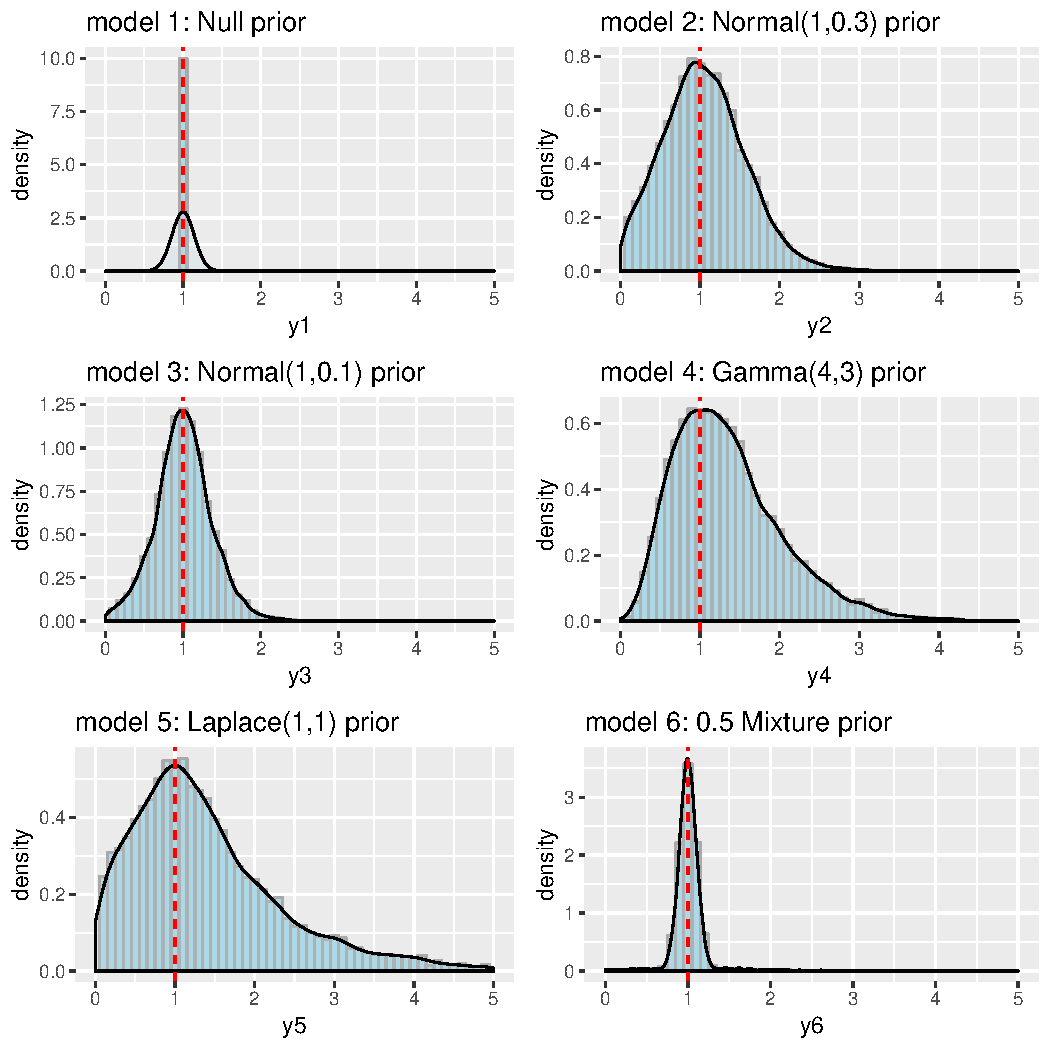
\includegraphics[width=1\linewidth]{../../R-codes/JAGS/plots/priordist}
	\caption{Histo-density plot of the prior probability distribution of proposed prior density models. The red dashed line indicates the center point of these distributions, which is 1.}
	\label{fig:priordist2}
\end{figure}

%---------------------------------------------------------------------------------------
Figure~\ref{fig:priordist2} show the distribution of $\lambda_{i,t}$ with hypothesised distributions just discussed, in histograms. Because we assign a prior distribution to our $\mu_{i,t}$ by directly multiplying by $\lambda_{i,t}$, the distribution of $\lambda_{i,t}$ is thought as the equivalent to the distribution of our prior. As presented in histograms, our priors have different distributions that suggest a different belief. Model 1 used a non-informative flat prior, that contains no information, and hence no distribution is observed, and only have 1 bar at 0. Model 2 used a $Normal(1, 0.3)$ prior that seems reasonable; however note that, because its left tail was truncated at 0, the distribution has lost its symmetrical property. Model 3 used a $Normal(1, 0.1)$ that has a smaller variance, hence the distribution is a little bit taller, indicating more observation tend to be close to the mean. Model 4 used a $Gamma(4, 3)$ prior; it skews towards the right-hand side. The distribution translates into that we are observing more positive anomalies compare to negative anomalies. Model 5 used a $Laplace(4, 3)$ prior, it also skews to the right, but with a heavier tail and a much higher distribution at extreme positive values, this translates into information at we are consistently observing a large anomaly. Lastly, we have model 6 that used a mixture prior; there is a very strong spike at 1 and some variation around it.

\subsection{Simulation setups }

In section 2.3, we present the results of the posterior distribution calculations for the synthesised data, with anomalies added on category AA on level 2 (leaf) of the hierarchy. The default setting for the data synthesis process is applied, with the addition of 25\% anomaly. An important note, the 25\% anomaly here meant an addition of 25\% of the count of category total on top of the hierarchy, not addition of 25\% on category AA. In mathematical terms, a 25\% anomaly would be equivalent to $1.25 y_{total,t}$. 

\subsection{Results}

\begin{table}[ht]
	\centering
	\begin{tabular}{crrrrrr}
		\hline
		Comparisons & Min. & 1st Qu. & Median & Mean & 3rd Qu. & Max. \\ 
		\hline
		M1:M2 & -2.126 & -1.574 & -0.599 & -0.868 & -0.158 & 0.113 \\ 
		M1:M3 & -4.456 & -3.295 & -2.069 & -2.032 & -0.650 & 0.189 \\ 
		M1:M4 & -2.992 & -1.729 & -1.174 & -1.303 & -0.800 & 0.106 \\ 
		M1:M5 & -2.645 & -1.745 & -0.764 & -1.172 & -0.590 & -0.124 \\ 
		M1:M6 & -3.383 & -2.200 & -1.645 & -1.683 & -1.047 & -0.258 \\ 
		M2:M3 & -4.555 & -2.288 & -1.884 & -1.164 & 0.713 & 1.440 \\ 
		M2:M4 & -2.393 & -1.009 & -0.552 & -0.434 & -0.155 & 2.232 \\ 
		M2:M5 & -2.382 & -0.494 & -0.071 & -0.304 & 0.267 & 0.782 \\ 
		M2:M6 & -3.331 & -1.571 & -0.626 & -0.815 & -0.122 & 1.639 \\ 
		M3:M4 & -2.450 & -0.285 & 0.895 & 0.730 & 1.787 & 3.658 \\ 
		M3:M5 & -1.020 & -0.578 & -0.168 & 0.860 & 2.345 & 3.677 \\ 
		M3:M6 & -1.995 & -1.322 & -0.412 & 0.349 & 1.649 & 4.198 \\ 
		M4:M5 & -1.884 & -0.905 & 0.501 & 0.131 & 0.913 & 2.282 \\ 
		M4:M6 & -2.858 & -1.537 & -0.829 & -0.380 & 1.029 & 2.039 \\ 
		M5:M6 & -3.259 & -0.929 & -0.672 & -0.511 & 0.378 & 1.454 \\ 
		\hline
	\end{tabular}
	\caption{DIC (with 1,000,000 iteration) summary distribution cross comparisons for model 1 to model 6} 
	\label{tab:dic1}
\end{table}

\newpage

Table~\ref{tab:dic1} gives the comparison of of DIC distributions. A comparison of M1: M2 indicated comparisons between model 1 and model 2, with DIC distribution of model 2 taking away the DIC distribution of model 1. An important note to take before the interpretation of results in this table is the weak signals (a negative value signals a model is better than another) of the DIC estimations. The initial DIC results with 1000 iterations give weak signals, showing signs of slow convergence, this meant that the absoulute DIC values for each model differ by a large margin each time DIC ran for different jags model. Due to convergence and size of numbers it is difficult for human eye to read the difference between numbers. Using the difference of values between models instead of absolute values of each model, sometimes we get negative mean and median values, and sometimes we get positive mean and median values, a negative value indicate second model is better than first model, and size of number indicate the size of difference, making it easier to interpret. Weak signals are still present when the number of iteration increase to 1,000,000. With repeated trials, Model 2 to model 6 consistently gives a lower DIC value compares to model 1, showing strong signals at 3rd Quartile and Max value. The observation provides strong evidence that Model 1 with non-informative prior gives the highest and worse DIC estimations out of all models. The DIC comparisons for model 2 to model 6 have weak signals on mean and median values, even with high iterations, and it is almost impossible to tell the difference, this suggests that there is no or close to no difference between the DIC values for model 2 to model 6. 

%-------------------------- Posterior dist total------------------------------------------------
\newpage %

\begin{table}[!ht]
	\centering
	\begin{tabular}{rrrrrrrr}
		\hline
		& mean & sd & 2.5\% & 50\% & 97.5\% & Rhat & n.eff \\ 
		\hline
		model 1 & 21.0615 & 0.0000 & 21.0615 & 21.0615 & 21.0615 &  & 0 \\ 
		model 2 & 24.4976 & 4.7805 & 15.7987 & 24.2398 & 34.1927 & 1 & 3119 \\ 
		model 3 & 24.3373 & 4.9322 & 15.7804 & 23.9781 & 34.8648 & 1 & 3009\\ 
		model 4 & 24.1116 & 4.8248 & 15.5574 & 23.7915 & 34.4035 & 1 & 3587 \\ 
		model 5 & 24.4041 & 4.9549 & 15.9001 & 24.1139 & 34.7204 & 1 & 3152 \\ 
		model 6 & 24.8840 & 4.9712 & 16.4075 & 24.5082 & 35.4618 & 1& 2895 \\ 
		\hline
	\end{tabular}
	\caption{Posterior distributions of different models for Total, with added anomalies, and calculated with independent Bayes model} 
	\label{tab:modelpost1}
\end{table}

\begin{figure}[!h]
	\centering
	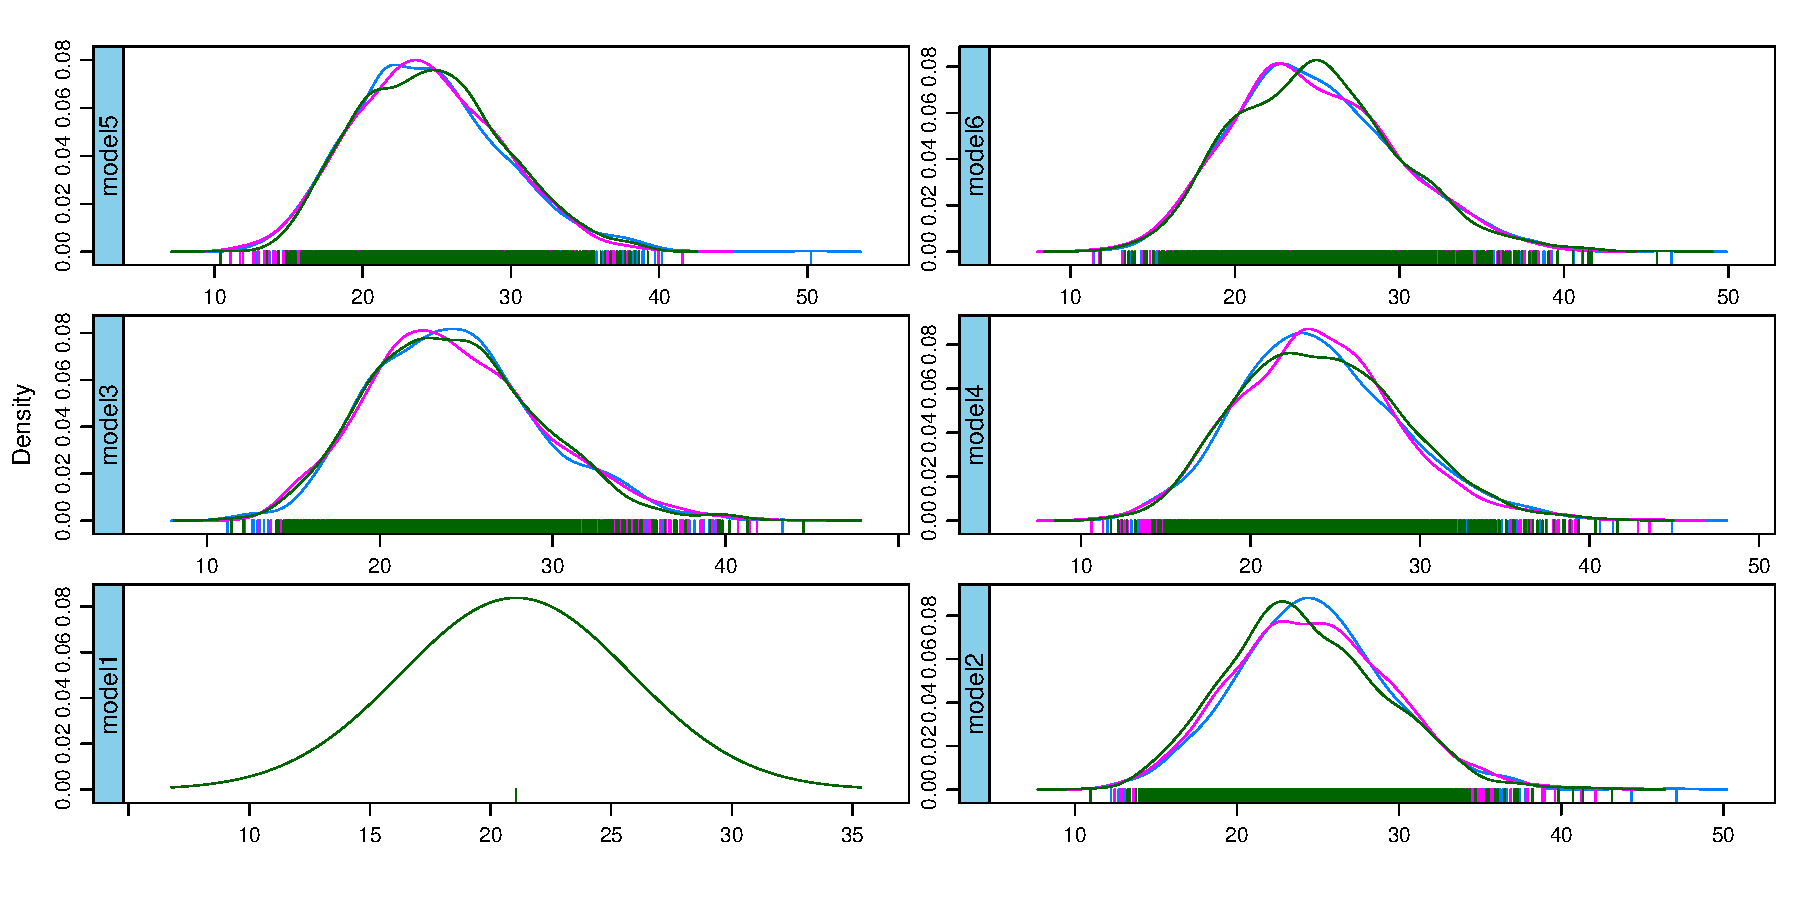
\includegraphics[width=1\linewidth]{../../R-codes/JAGS/plots/findmodel/Densitytotal3abn}
	\caption{Posterior distributions of different models for Total, with added anomalies, and calculated with independent Bayes model}
	\label{fig:densitytotal3abn}
\end{figure}

Table~\ref{tab:modelpost1} and figure~\ref{fig:densitytotal3abn} gives the posterior distribution of the category total, for each of the model. Model 1 uses non-informative prior, and it gives the most particular posterior out of all models at level 0 (total), the mean value of the posterior distribution is around 4.5 unit lower than other models, there is no standard deviation, and the number of effective samples is 0. Our observation suggests that non-informative priors produce a significantly different result compares to weakly informative priors. Posterior distributions for model 2 to model 6 are very similar and very hard to tell any significant difference, other than there seems to be a large difference between the number of effective sample size.

\newpage %----------------------------Posterior dist A ----------------------------------------------
\begin{table}[!ht]
	\centering
	\begin{tabular}{rrrrrrrr}
		\hline
		& mean & sd & 2.5\% & 50\% & 97.5\% & Rhat & n.eff \\ 
		\hline
		model 1 & 10.5463 & 0.0000 & 10.5463 & 10.5463 & 10.5463 &  & 0 \\ 
		model 2 & 12.3481 & 3.5241 & 6.4608 & 12.0826 & 19.7636 & 1 & 2833 \\ 
		model 3 & 12.2433 & 3.5058 & 6.3331 & 11.9460 & 20.1100 & 1 & 2955 \\ 
		model 4 & 12.0331 & 3.2668 & 6.4515 & 11.7501 & 19.1090 & 1 & 3322 \\ 
		model 5 & 12.3475 & 3.5362 & 6.4799 & 12.0049 & 19.9832 & 1 & 2503 \\ 
		model 6 & 12.9588 & 3.6536 & 6.8353 & 12.6056 & 21.2272 & 1 & 3000 \\ 
		\hline
	\end{tabular}
	\caption{Posterior distributions of different models for A , with added anomalies, and calculated with independent Bayes model} 
	\label{tab:modelpost2}
\end{table}

\begin{figure}[!h]
	\centering
	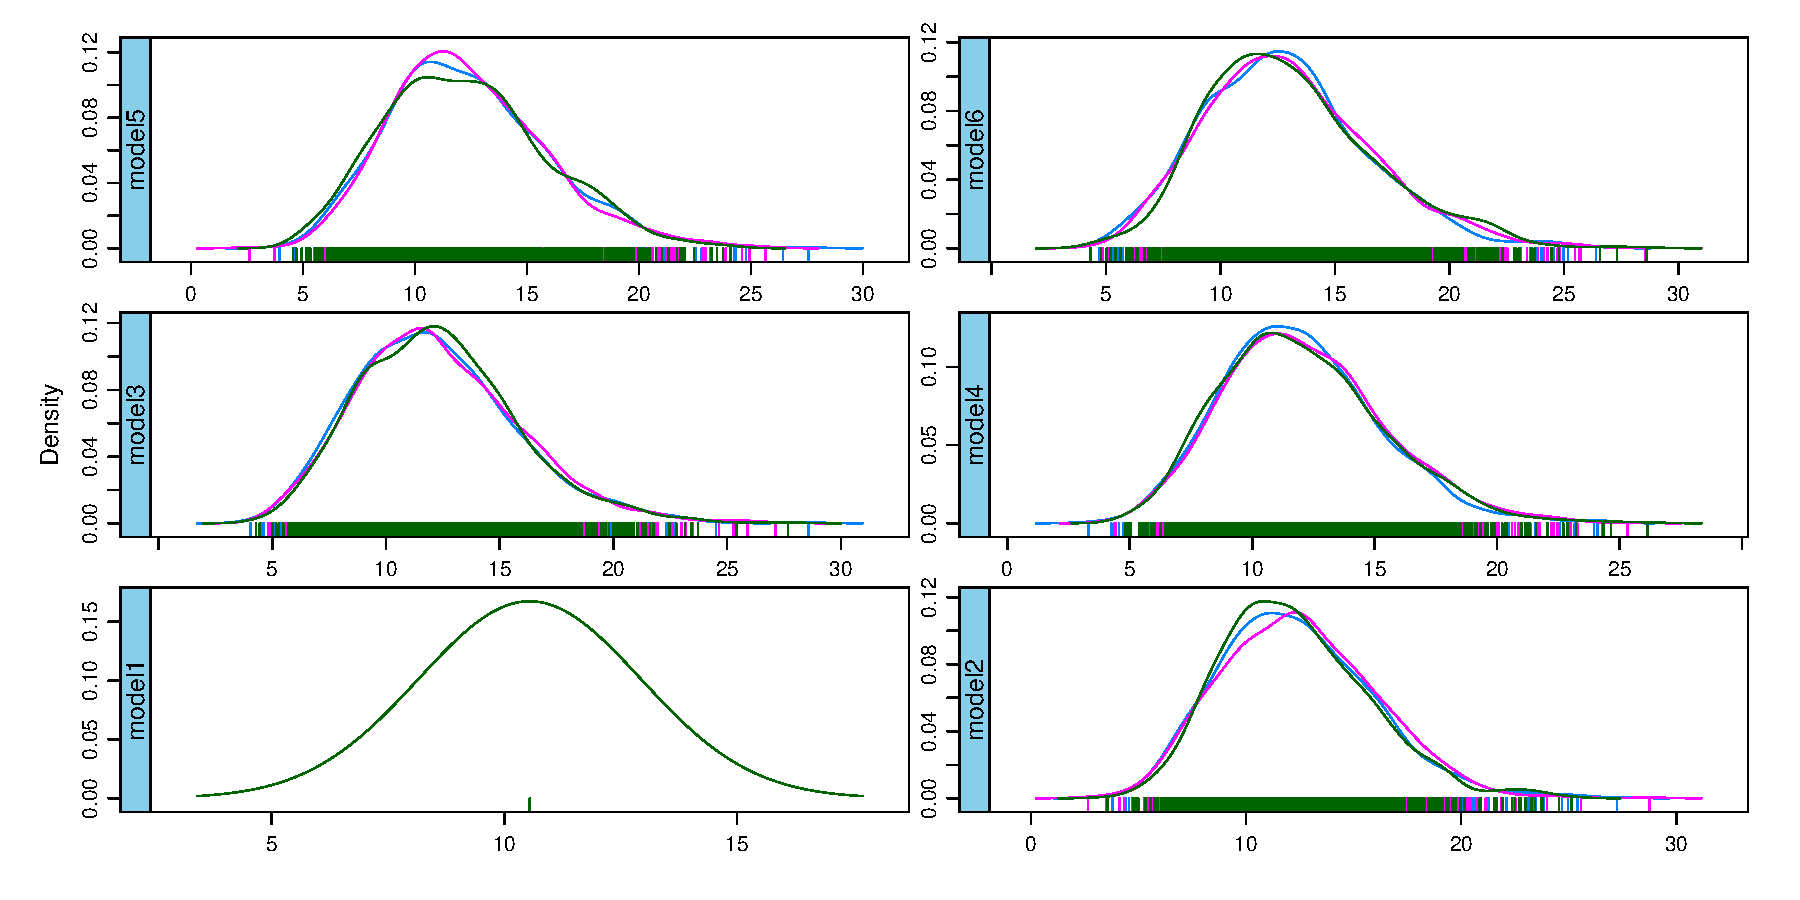
\includegraphics[width=1\linewidth]{../../R-codes/JAGS/plots/findmodel/DensityA3abn}
	\caption{Posterior distributions of different models for A , with added anomalies, and calculated with independent Bayes model}
	\label{fig:densityA3abn}
\end{figure}

Table~\ref{tab:modelpost2} and figure~\ref{fig:densityA3abn} gives the posterior distribution of the category A, for each of the model. Model 1 uses non-informative prior, and it gives the most particular posterior out of all models at level 1 (A), the mean value of the posterior distribution is around 2 unit lower than other models, there is no standard deviation, and the number of effective samples is 0. Our observation suggests that non-informative priors produce a significantly different result compares to weakly informative priors. Posterior distributions for model 2 to model 6 are very similar and very hard to tell any significant difference, other than there seems to be a large difference between the number of effective sample size.

\newpage %--------------------------- Posterior dist AA -----------------------------------------------
\begin{table}[!ht]
	\centering
	\begin{tabular}{rrrrrrrr}
		\hline
		& mean & sd & 2.5\% & 50\% & 97.5\% & Rhat & n.eff \\ 
		\hline
		model 1 & 5.2477 & 0.0000 & 5.2477 & 5.2477 & 5.2477 &  & 0 \\ 
		model 2 & 7.4081 & 2.7444 & 2.8634 & 7.1136 & 13.3165 & 1 & 2273 \\ 
		model 3 & 7.3234 & 2.7423 & 2.8910 & 7.0234 & 13.3408 & 1 & 2372 \\ 
		model 4 & 6.9192 & 2.4111 & 3.0404 & 6.6744 & 12.3585 & 1 & 3000 \\ 
		model 5 & 7.6640 & 2.8689 & 3.0550 & 7.2466 & 14.0954 & 1 & 1886 \\ 
		model 6 & 7.8524 & 2.7397 & 3.4434 & 7.5279 & 14.0425 & 1 & 2856 \\ 
		\hline
	\end{tabular}
	\caption{Posterior distributions of different models for AA, with added anomalies, and calculated with independent Bayes model} 
	\label{tab:modelpost3}
\end{table}

\begin{figure}[!h]
	\centering
	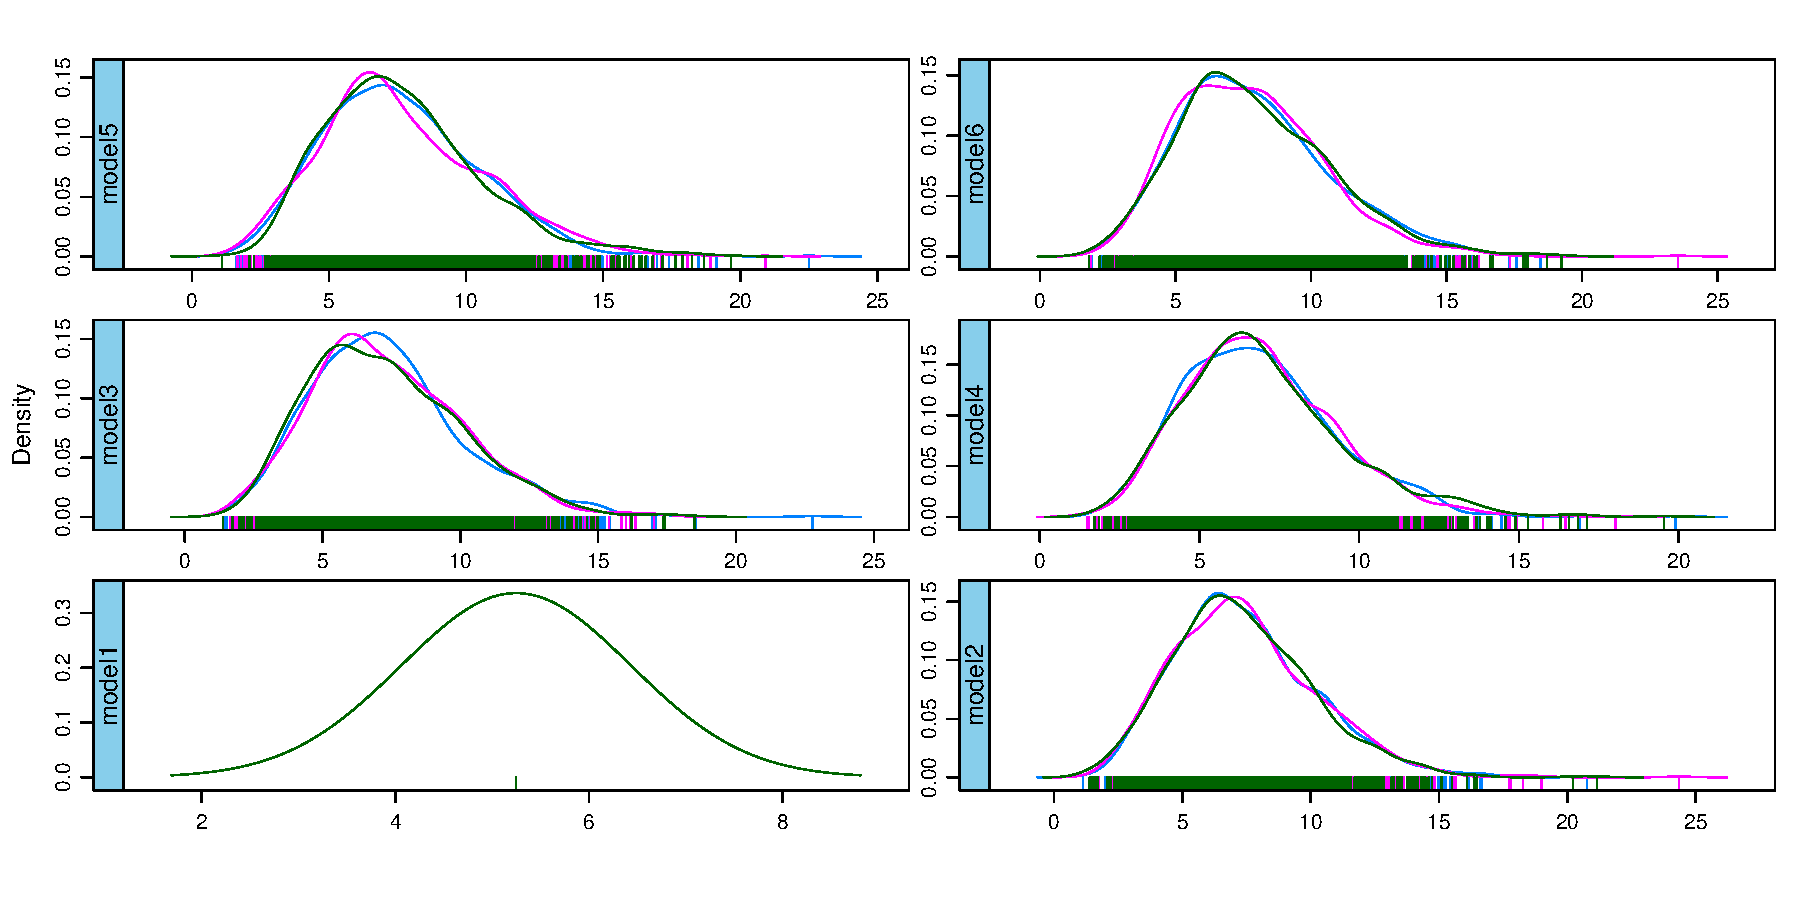
\includegraphics[width=1\linewidth]{../../R-codes/JAGS/plots/findmodel/DensityAA3abn}
	\caption{Posterior distributions of different models for AA, with added anomalies, and calculated with independent Bayes model}
	\label{fig:densityAA3abn}
\end{figure}

Table~\ref{tab:modelpost3} and figure~\ref{fig:densityAA3abn} gives the posterior distribution of the category AA, for each of the model. Model 1 uses non-informative prior, and it gives the most particular posterior out of all models at level 2 (AA), the mean value of the posterior distribution is around 2 unit lower than other models, there is no standard deviation, and the number of effective samples is 0. Our observation suggests that non-informative priors produce a significantly different result compares to weakly informative priors. Posterior distributions for model 2 to model 6 are very similar and very hard to tell any significant difference, other than there seems to be a large difference between the number of effective sample size.

\newpage

Considering posterior distribution results of all three hierarchical levels, it is apparent that Model 1 gives a significantly different posterior compares to all other models, suggesting that the usage of non-informative prior will generate significantly different results compares to weakly informative priors at all levels of Hierarchy. Model 2 to model 6 gives similar posterior distribution, with similar numeric values in tables and similar shapes in density plots in all levels, this suggests that there no or close to no differences between the posterior distributions of Model 2 to model 6 and using slightly different weakly informative prior does not make a significant impact on our posterior distribution results in all levels of hierarchy. The mean and standard deviation of posteriors for model 2 to model 6 decreases as the level of hierarchy increase (going down the hierarchy), with category total having the largest mean and standard deviation, category A having smaller mean and standard deviation, and category AA having the smallest mean and deviation. Our observation makes sense as the aggregation constraints of hierarchical datasets dictates that the mean and sample size of categories at higher hierarchy will always be greater than mean and sample size of categories at the lower hierarchy. The number of effective size for model 2 to 6 seem to decrease as the level of hierarchy increase, which made sense because due to aggregation constraints, observed values at a lower hierarchy tend to be smaller and less variable, and this will produce a stronger autocorrelation during the MCMC process. 

%-------------------------- TRACE Plots ------------------------------------
\newpage 

\begin{figure}[!ht]
	\centering
	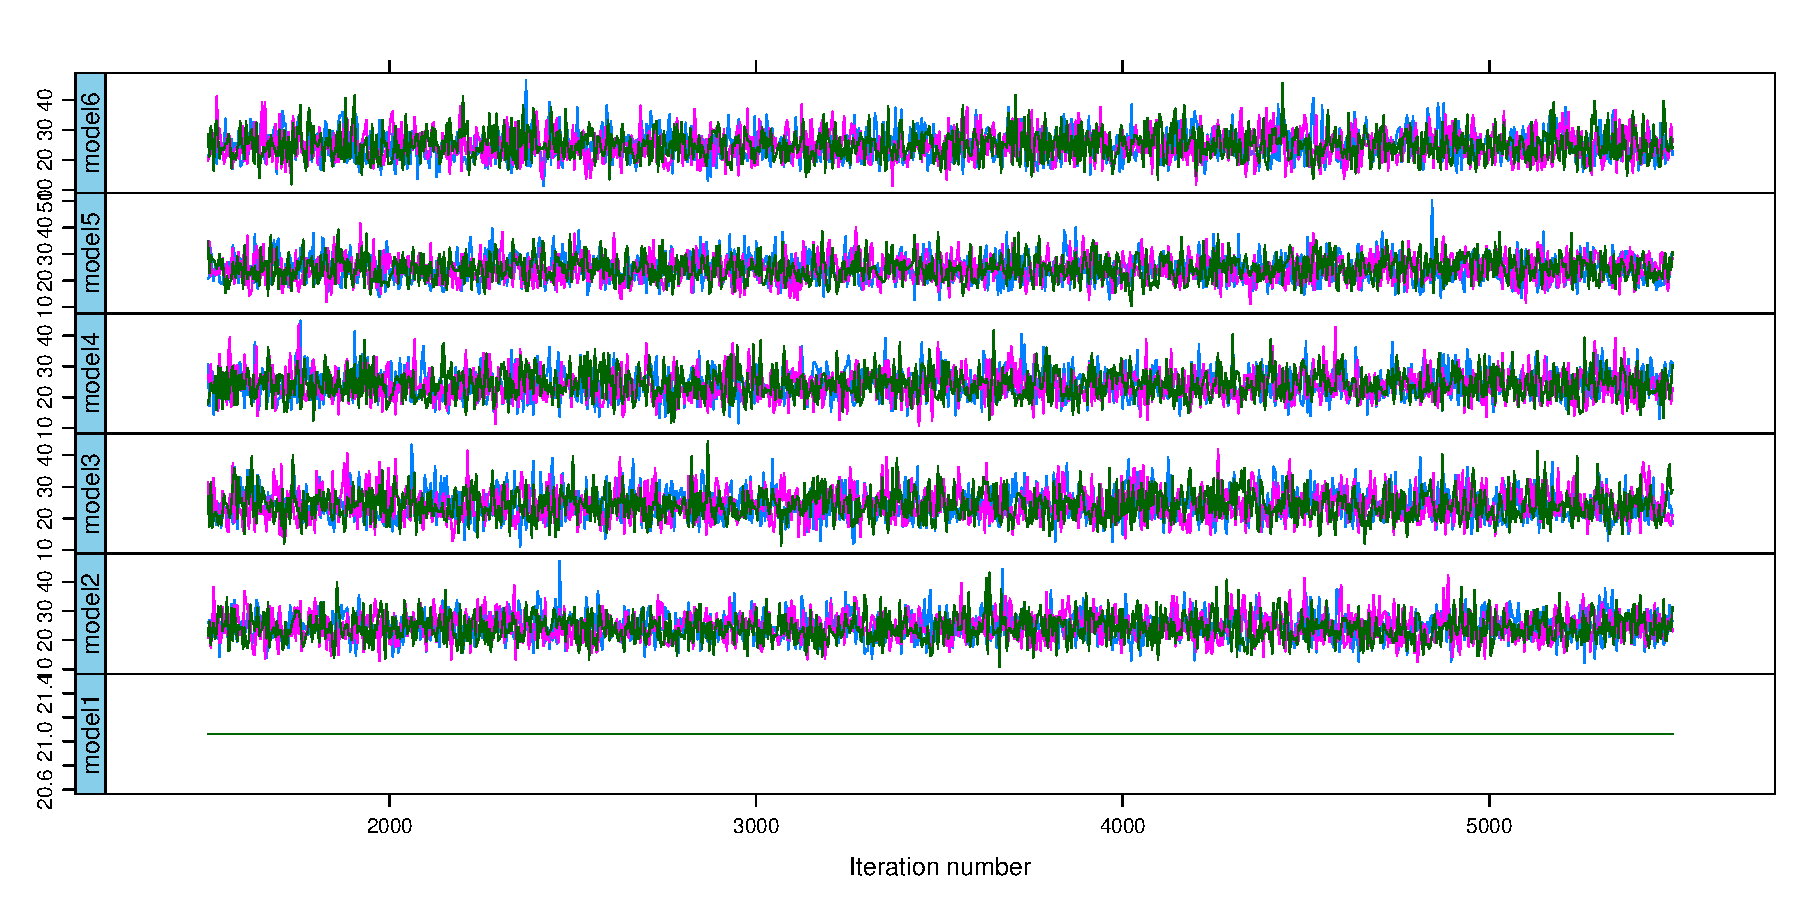
\includegraphics[width=1.0\linewidth]{../../R-codes/JAGS/plots/findmodel/Tracetotal3abn.PDF}
	\caption{Traces plot for category total of model 1 to model 6}
	\label{fig:tracetotal}
\end{figure}

\begin{figure}[!ht]
	\centering
	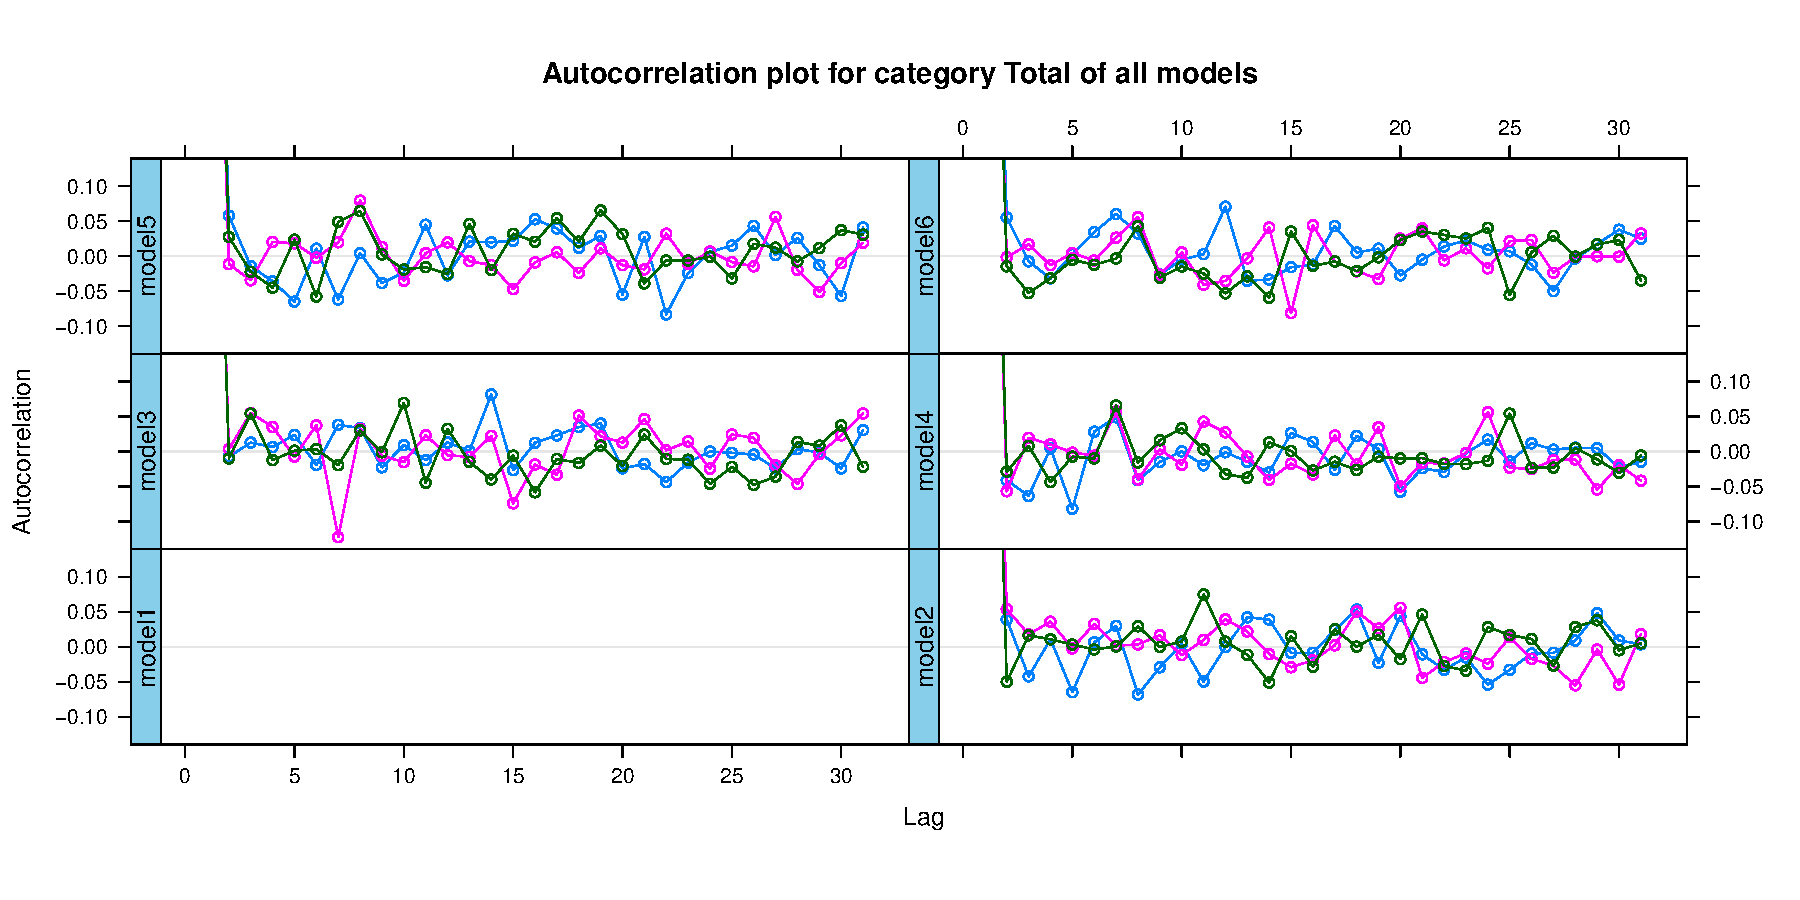
\includegraphics[width=1.0\linewidth]{../../R-codes/JAGS/plots/findmodel/Acftotal3abn.PDF}
	\caption{ACF plots for category total of model 1 to model 6}
	\label{fig:ACFtotal}
\end{figure}

Trace plots in figure~\ref{fig:tracetotal} allows a visual inspection of convergence at the top level of the hierarchy. The trace plot for model 1 is completely flat, suggesting that there is no mixing at all ( we have a fixed parameter), and trace plots for model 2 to 6 vary around the mean and do not show any trend, this suggest that our samples have mixed well and chains have converged. The Auto Correlation Function (ACF) plots presented in figure~\ref{fig:ACFtotal} gives no ACF for model 1; this indicates that model 1 gives no autocorrelation. ACF plots for model 2 to model 6 shows no signs of significant autocorrelation. 

\newpage %Z--------------------------------------------------------------

\begin{figure}[!ht]
	\centering
	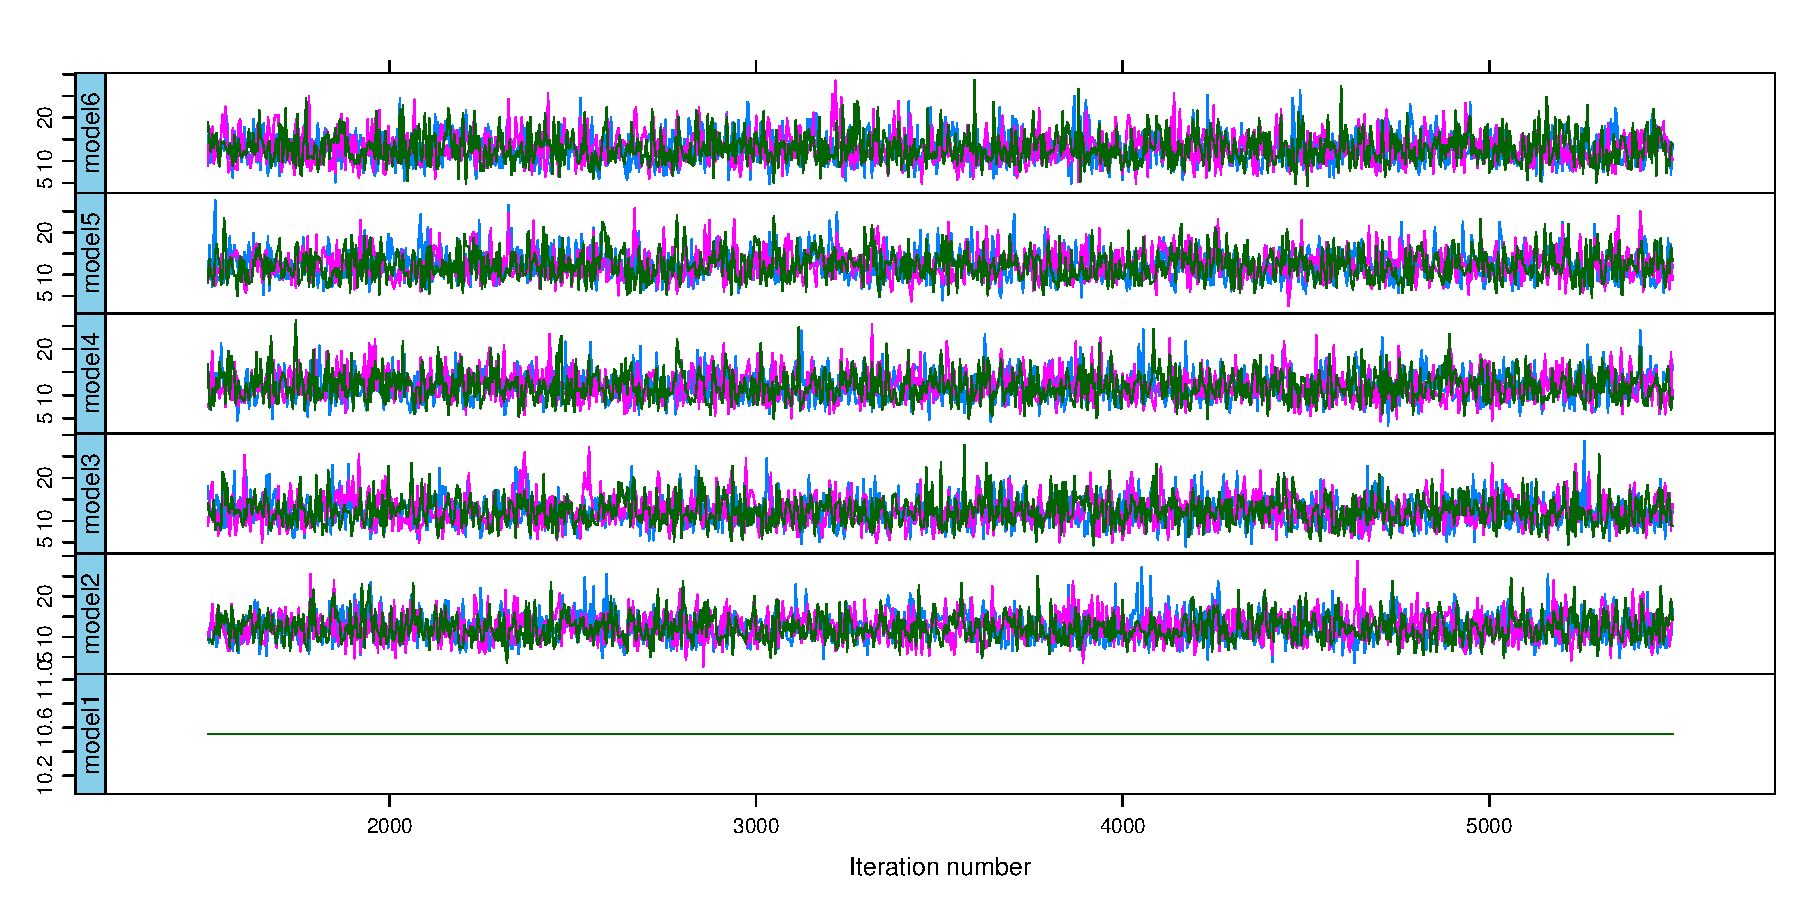
\includegraphics[width=1.0\linewidth]{../../R-codes/JAGS/plots/findmodel/TraceA3abn.PDF}
	\caption{Traces plot for category A of model 1 to model 6}
	\label{fig:traceA}
\end{figure}

\begin{figure}[!ht]
	\centering
	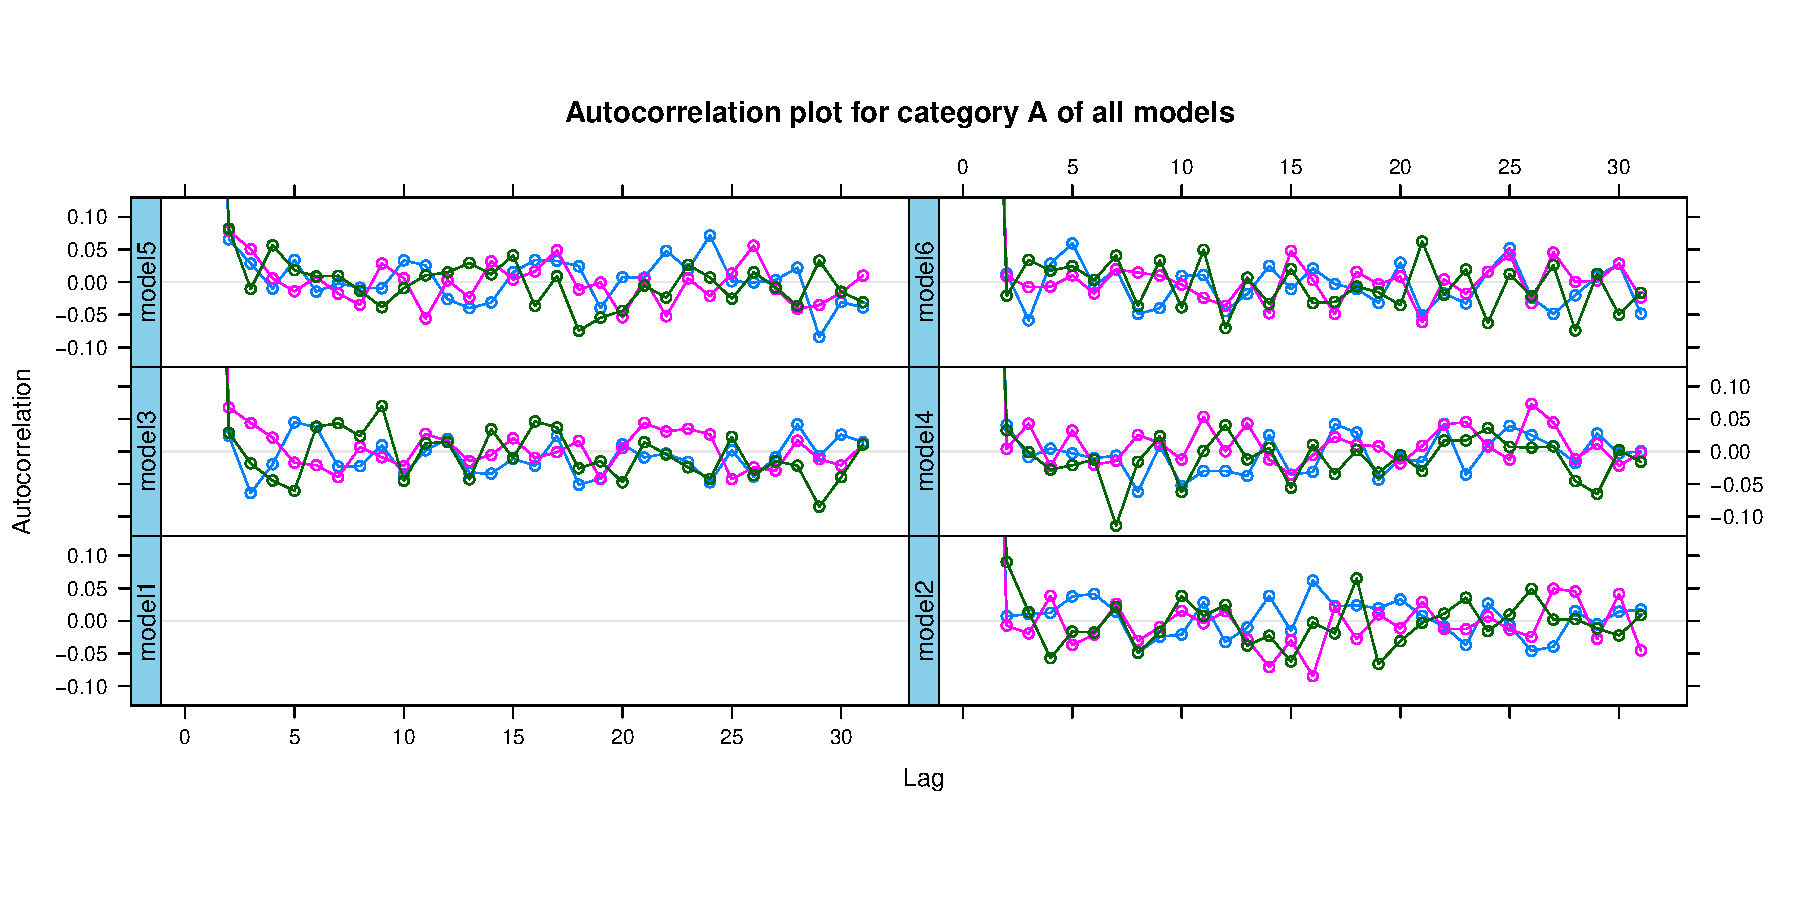
\includegraphics[width=1.0\linewidth]{../../R-codes/JAGS/plots/findmodel/AcfA3abn.PDF}
	\caption{ACFs plot for category A of model 1 to model 6}
	\label{fig:ACFA}
\end{figure}

Trace plots in figure~\ref{fig:traceA} allows a visual inspection of convergence at the second level of the hierarchy. The trace plot for model 1 is completely flat, suggesting that there is no mixing at all, and trace plots for model 2 to 6 vary around the mean and do not show any trend, this suggest that our samples have mixed well and chains have converged. The Auto Correlation Function (ACF) plots presented in figure~\ref{fig:ACFA} gives no ACF for model 1. Our observation indicates that model 1 gives no autocorrelation. ACF plots for model 2 to model 6 shows no signs of significant autocorrelation. 

\newpage %Z--------------------------------------------------------------

\begin{figure}[!ht]
	\centering
	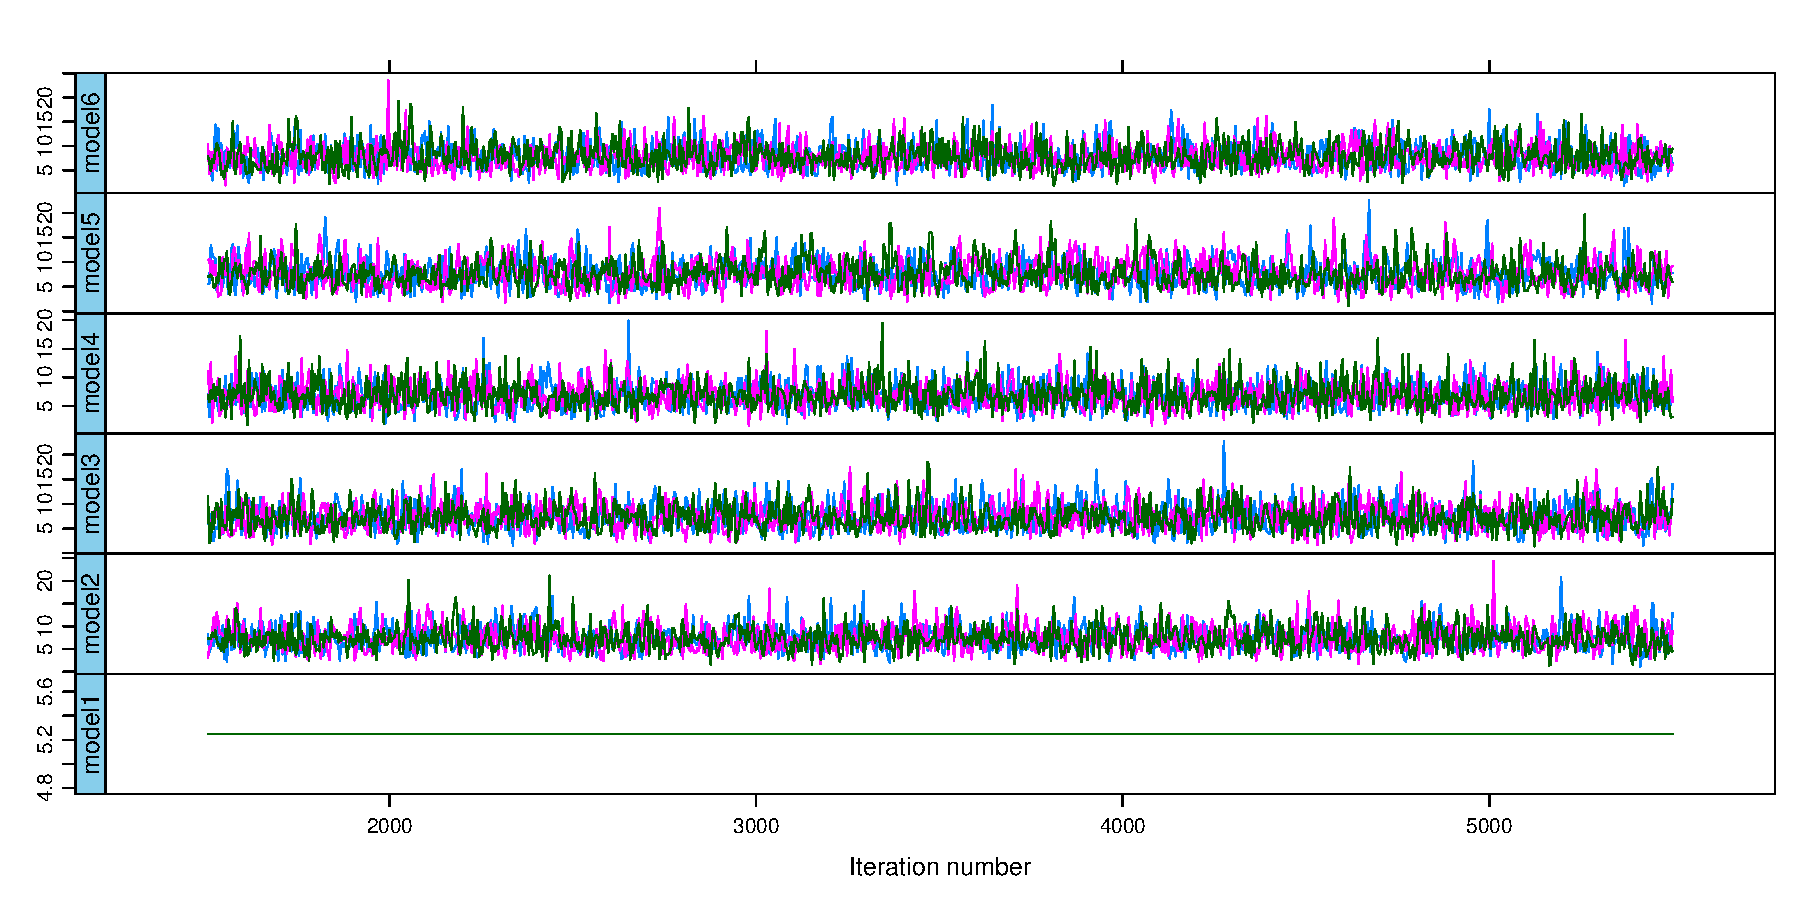
\includegraphics[width=1.0\linewidth]{../../R-codes/JAGS/plots/findmodel/TraceAA3abn.PDF}
	\caption{Traces plot for category AA of model 1 to model 6}
	\label{fig:traceAA}
\end{figure}

\begin{figure}[!ht]
	\centering
	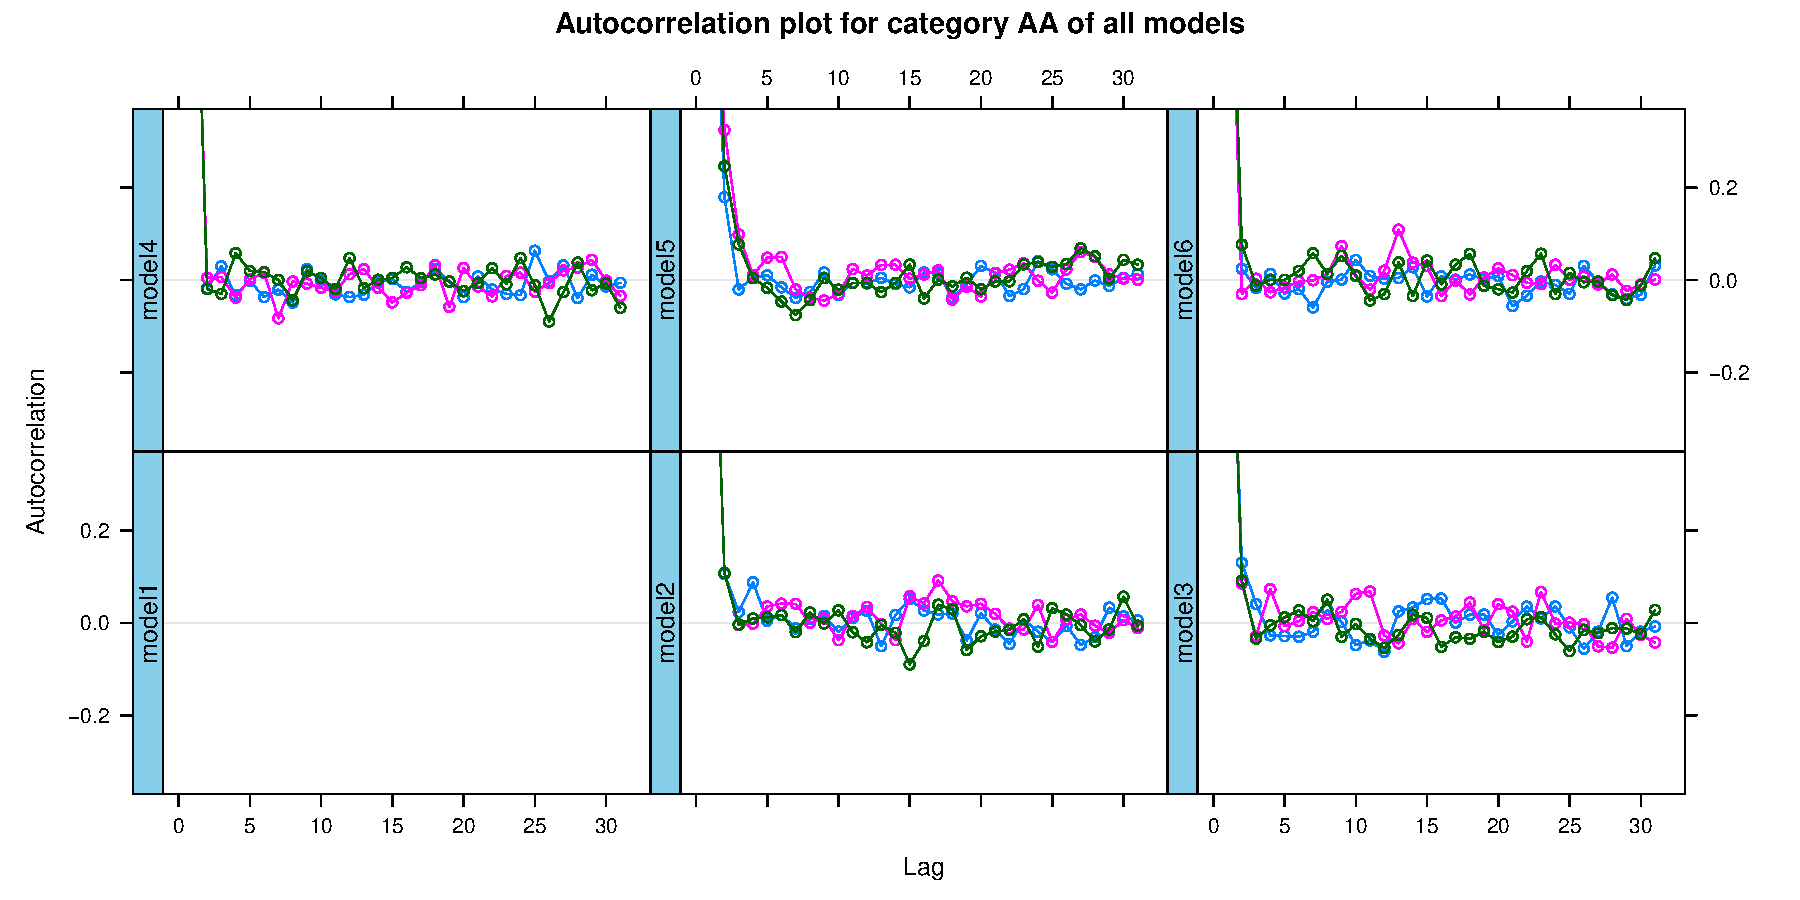
\includegraphics[width=1.0\linewidth]{../../R-codes/JAGS/plots/findmodel/AcfAA3abn.PDF}
	\caption{ACFs plot for category AA of model 1 to model 6}
	\label{fig:ACFAA}
\end{figure}

Trace plots in figure~\ref{fig:traceAA} allows a visual inspection of convergence at the second level of the hierarchy. The trace plot for model 1 is completely flat, suggesting that there is no mixing at all, and trace plots for model 2 to 6 vary around the mean and do not show any trend, this suggest that our samples have mixed well and chains have converged. The Auto Correlation Function (ACF) plots presented in figure~\ref{fig:ACFAA} gives no ACF for model 1; this indicates that model 1 gives no autocorrelation. ACF plots for model 2 to model 6 shows a weak sign of autocorrelation. 

\newpage

Considering trace plots and ACF plots results of all three hierarchical levels, we observe no strong correlation at all levels of hierarchy. However, there seems to be a slight increase in autocorrelation at lower levels of hierarchy. The is indicate that categories at lower hierarchy mixes slower compare to categories at the higher hierarchy.

\subsection{Discussion}

As expected, models that used weakly-informed priors had outperformed the model with non-informative prior, in terms of model goodness-of-fit, this highlighted the importance of assigning a prior distribution for Bayesian calculations and we should at least provide some distribution to our prior, even if it is just a flat uniform prior (which is also considered as a non-informative prior). Different hypothesised weakly-informed priors performed similarly, and we were unable to detect a significant difference between our priors from the DIC comparisons, and we did not observe significant differences in posterior distributions. If there is no evidence suggesting a prior is better than another prior, how do we decide which prior is preferable? The reasonable idea is that we should use the simplest prior, so complex priors such as the mixture prior and Laplace prior is out of the question. Especially for the case of Hierarchical Bayesian Model (HBM), we would want to build our HBM with the simplest prior as possible. Otherwise, our model would be extremely complex and hard to build. Hence, a Normal(1,0.3) prior is used for the rest of our simulations. A model with normal distributions is simple and suitable for observations with large samples as indicated by Central limit theorem (CLT) theorem. The essential idea is that weakly informative prior should contain enough information to regularize, this means that the prior should rule out unreasonable parameter values but is not so strong as to rule out values that might make sense. The might be other considerations as well, for example the Stan Development Team favour the lighter tails of a weakly informative prior with a Gaussian shape as the most robust default prior for it's accurate and fast statistical computation and ease of optimising the scale \citep{stan2018}, and \citet{gelman2006prior} suggested the usage of half-Cauchy prior distribution for observations with small values. 

\newpara

Another interesting find from this simulation is that uncertainty in Bayesian estimations will cause uncertainty in DIC results, and it is tough to confidently decide which model is the best if there is no substantial difference between the performance of models. Increasing the iteration number help a bit, but does not eliminate the problem and uncertainty still exists. A possible alternative to DIC is (Watanabe-Akaike information criteria), but it relies on a data partition that would cause difficulties with structured models \citep{gelman2014understanding}. Cross-validation could also work, but for Bayesian stats, it will be computationally expensive. Our results agree with conclusions from \citet{gelman2014understanding}, that predictive error comparisons (such as DIC) does work for highly dissimilar models, but have a weak performance for similar models, and sometimes it is challenging to draw significant conclusions.

%===============================================================================================================

\section{Simulation 2: Anomaly}

\subsection{Simulation setups}

In section 2.4, we present the results of the posterior distribution calculations for the synthesised data, with different increments of anomalies added on category AA on level 2 (leaf) of the hierarchy. The default setting for the data synthesis and anomaly addition process is applied for each scenario, with the addition of 0\%, 10\%, 25\%, 50\%, 100\%, 250\% and 500\% anomaly. An important note, the 25\% anomaly here meant an addition of 25\% of the count of category total ($\sum_i \mu_{i,t}$) on top of the hierarchy, not addition of 25\% on category AA.  

\subsection{Rsults}
\begin{table}[ht]
	\centering
	\begin{tabular}{crrrrrr}
		\hline
		Anomaly &&&&&&\\
		(\% of total) & Min. & 1st Qu. & Median & Mean & 3rd Qu. & Max. \\ 
		\hline
		0 & -0.466 & 0.188 & 0.437 & 0.545 & 0.955 & 1.556 \\ 
		10 & -1.910 & -0.693 & 0.876 & 1.144 & 1.894 & 6.640 \\ 
		25 & -6.274 & -3.079 & -1.966 & -1.984 & -0.658 & 1.825 \\ 
		50 & -4.352 & -1.185 & -0.038 & -0.385 & 0.823 & 2.420 \\ 
		100 & -5.074 & -1.096 & 0.323 & -0.383 & 1.194 & 1.873 \\ 
		250 & -1.813 & -1.657 & -0.917 & -0.181 & 0.546 & 3.681 \\ 
		500 & -4.416 & -1.678 & -0.613 & -0.875 & 0.430 & 1.401 \\ 
		\hline
	\end{tabular}
	\caption{DIC (with 1,000,000 iteration) comparisons between Independent Bayes model and Hierarchical Bayes model (HBM -IBM) for different anomalies sizes} 
	\label{tab:dicanomaly}
\end{table}

Table~\ref{tab:dicanomaly} gives the comparison of DIC distributions of Independent Bayesian Model (IBM) and Hierarchical Bayesian Model (HBM) for scenarios with different increments of anomaly added. For all scenarios, the mean and median value is mostly negative; the negative signals suggest that HBM seem to perform better than IBM, most of the time. Uncertainty in Bayesian estimations still exist and have impacts on the reliability of our DIC comparison, although we mostly see negative values for median and mean of the DIC difference distribution, the signal still shifts every time our JAGS model is re-run. Our observation suggests that although there might be a difference between IBM and HBM, it might not be a very big difference.  

\begin{table}[ht]
	\centering
	\begin{tabular}{rrrrrrrr}
		\hline
		& mean & sd & 2.5\% & 50\% & 97.5\% & Rhat & n.eff \\ 
		\hline
		Anomaly0 & 19.1481 & 4.2840 & 11.7152 & 18.8136 & 28.3845 & 1 & 3000 \\ 
		Anomaly10 & 21.4084 & 4.7272 & 13.1528 & 21.0041 & 31.6607 & 1 & 3000 \\ 
		Anomaly25 & 24.4356 & 4.9374 & 16.0687 & 24.0399 & 34.7248 & 1 & 2975 \\ 
		Anomaly50 & 30.2932 & 5.3613 & 20.8844 & 29.8973 & 41.9325 & 1 & 2912 \\ 
		Anomaly100 & 40.4338 & 6.1531 & 29.3330 & 40.0987 & 53.8314 & 1 & 2889 \\ 
		Anomaly250 & 71.9683 & 8.4372 & 56.5531 & 71.6763 & 89.4346 & 1 & 3000 \\ 
		Anomaly500 & 122.4365 & 10.7971 & 101.9952 & 122.2718 & 144.5457 & 1 & 3132 \\ 
		\hline
	\end{tabular}
	\caption{Posterior distributions of different models for Total, with different increments of added anomalies, and calculated with independent Bayes model} 
	\label{tab:pstanototal}
\end{table}

\begin{table}[ht]
	\centering
	\begin{tabular}{rrrrrrrr}
		\hline
		& mean & sd & 2.5\% & 50\% & 97.5\% & Rhat & n.eff \\ 
		\hline
		Anomaly0 & 19.3114 & 4.4361 & 11.5960 & 18.9555 & 28.9686 & 1 & 2934 \\ 
		Anomaly10 & 21.3883 & 4.5971 & 13.3033 & 21.1152 & 31.2900 & 1 & 2799 \\ 
		Anomaly25 & 24.3800 & 4.9083 & 15.8281 & 24.1057 & 34.9855 & 1 & 3000 \\ 
		Anomaly50 & 30.5664 & 5.4857 & 20.7071 & 30.2800 & 42.3242 & 1 & 2713 \\ 
		Anomaly100 & 40.5794 & 6.2480 & 29.1623 & 40.2459 & 53.0399 & 1 & 2704 \\ 
		Anomaly250 & 72.0177 & 8.2580 & 57.1126 & 71.8129 & 88.7105 & 1 & 2723 \\ 
		Anomaly500 & 121.9641 & 10.3188 & 102.7605 & 121.6646 & 142.4118 & 1 & 2173 \\ 
		\hline
	\end{tabular}
	\caption{Posterior distributions of different models for Total, with different increments of added anomalies, and calculated with Hierarchical Bayes model} 
	\label{tab:pstanototal2}
\end{table}

Table~\ref{tab:pstanototal} and table~\ref{tab:pstanototal2} gives the posterior distribution of the category total, with different increments of anomalies added, for IBM and HBM. There are differences between the mean and standard deviations of posteriors of IBM and HBM, but it is very small and very hard to tell. However, for HBM The number of Effective Sample Size (ESS) for HBM posteriors seem to be overall less than IBM posteriors, this suggests that values observed in total category on top of the hierarchy level for HBM are overall less independent than BM. As the size of the anomaly increases, the number of ESS tend to decrease. 

\newpage

\begin{table}[ht]
	\centering
	\begin{tabular}{rrrrrrrr}
		\hline
		& mean & sd & 2.5\% & 50\% & 97.5\% & Rhat & n.eff \\ 
		\hline
		Anomaly0 & 7.1758 & 2.7278 & 3.0586 & 6.7391 & 13.6749 & 1 & 2844 \\ 
		Anomaly10 & 9.3215 & 3.1367 & 4.1286 & 8.9552 & 16.3998 & 1 & 2630 \\ 
		Anomaly25 & 12.3410 & 3.5655 & 6.4488 & 11.9857 & 20.3604 & 1 & 3038 \\ 
		Anomaly50 & 18.4421 & 4.3162 & 10.8431 & 18.1170 & 27.7122 & 1 & 2839 \\ 
		Anomaly100 & 28.3032 & 5.3432 & 19.1588 & 27.8652 & 40.0187 & 1 & 3008 \\ 
		Anomaly250 & 58.6906 & 7.3628 & 45.1079 & 58.6335 & 73.7809 & 1 & 2118 \\ 
		Anomaly500 & 104.7585 & 9.5672 & 87.1657 & 104.5580 & 123.4846 & 1 & 2235 \\ 
		\hline
	\end{tabular}
	\caption{Posterior distributions of different models for A , with different increments of added anomalies, and calculated with Independent Bayes model} 
	\label{tab:pstanoA}
\end{table}

\begin{table}[ht]
	\centering
	\begin{tabular}{rrrrrrrr}
		\hline
		& mean & sd & 2.5\% & 50\% & 97.5\% & Rhat & n.eff \\ 
		\hline
		Anomaly0 & 7.1740 & 2.7263 & 2.8494 & 6.8467 & 13.2835 & 1 & 2559 \\ 
		Anomaly10 & 9.1731 & 3.0292 & 4.1612 & 8.8307 & 15.8837 & 1 & 2961\\ 
		Anomaly25 & 12.4274 & 3.6049 & 6.3125 & 12.0656 & 20.2620 & 1 & 2703 \\ 
		Anomaly50 & 18.5048 & 4.3162 & 10.9271 & 18.2437 & 28.0090 & 1 & 2580 \\ 
		Anomaly100 & 28.6123 & 5.2341 & 19.2090 & 28.1992 & 39.9182 & 1 & 2370 \\ 
		Anomaly250 & 59.6236 & 7.2375 & 46.4370 & 59.4535 & 74.8256 & 1 & 1940 \\ 
		Anomaly500 & 107.9043 & 9.7689 & 89.7498 & 107.4554 & 129.0404 & 1 & 1338 \\ 
		\hline
	\end{tabular}
	\caption{Posterior distributions of different models for A , with different increments of added anomalies, and calculated with Hierarchical Bayes model} 
	\label{tab:pstanoA2}
\end{table}

Table~\ref{tab:pstanoA} and table~\ref{tab:pstanoA2} gives the posterior distribution of the category A, with different increments of anomalies added, for IBM and HBM. There are also differences between the mean and standard deviations of posteriors of IBM and HBM, but it is also very small and very hard to tell. The number of ESS for HBM posteriors seem to be overall less than IBM posteriors. Our observation suggests that values observed in A category on second of the hierarchy level for HBM are overall less independent than BM. As the size of the anomaly increases, the number of ESS tend to decrease. 

\newpage

\begin{table}[ht]
	\centering
	\begin{tabular}{rrrrrrrr}
		\hline
		& mean & sd & 2.5\% & 50\% & 97.5\% & Rhat & n.eff \\ 
		\hline
		Anomaly0 & 2.3062 & 1.4859 & 0.4009 & 2.0034 & 6.0143 & 1 & 2401 \\ 
		Anomaly10 & 4.2976 & 2.1384 & 1.2137 & 3.8992 & 9.5420 & 1 & 2461 \\ 
		Anomaly25 & 7.4243 & 2.8041 & 2.8709 & 7.0744 & 13.8003 & 1 & 2214\\ 
		Anomaly50 & 13.3455 & 3.5920 & 7.3160 & 13.0175 & 21.0238 & 1 & 2428 \\ 
		Anomaly100 & 22.4374 & 4.5194 & 14.6914 & 22.0898 & 31.9623 & 1 & 2029 \\ 
		Anomaly250 & 48.8502 & 6.1544 & 37.2238 & 48.5964 & 61.2842 & 1 & 1568 \\ 
		Anomaly500 & 100.5322 & 11.0472 & 79.0267 & 100.3259 & 122.1376 & 1 & 1115 \\ 
		\hline
	\end{tabular}
	\caption{Posterior distributions of different models for AA, with different increments of added anomalies, and calculated with Independent Bayes model} 
	\label{tab:pstanoAA}
\end{table}

\begin{table}[ht]
	\centering
	\begin{tabular}{rrrrrrrr}
		\hline
		& mean & sd & 2.5\% & 50\% & 97.5\% & Rhat & n.eff \\ 
		\hline
		Anomaly0 & 2.1538 & 1.4960 & 0.3505 & 1.7838 & 6.1010 & 1 & 2073 \\ 
		Anomaly10 & 4.3301 & 2.1448 & 1.1920 & 3.9651 & 9.5508 & 1 & 2046 \\ 
		Anomaly25 & 7.6847 & 2.8131 & 3.0945 & 7.3379 & 13.8861 & 1 & 2149 \\ 
		Anomaly50 & 13.6061 & 3.6369 & 7.2589 & 13.3337 & 21.4732 & 1 & 2054 \\ 
		Anomaly100 & 23.0253 & 4.5067 & 14.9764 & 22.7288 & 32.6668 & 1 & 1679 \\ 
		Anomaly250 & 51.9695 & 6.3876 & 40.2516 & 51.8076 & 65.5484 & 1 & 951 \\ 
		Anomaly500 & 96.0807 & 9.1704 & 79.5825 & 95.8225 & 115.7111 & 1& 951 \\ 
		\hline
	\end{tabular}
	\caption{Posterior distributions of different models for AA, with different increments of added anomalies, and calculated with Hierarchical Bayes model} 
	\label{tab:pstanoAA2}
\end{table}

Table~\ref{tab:pstanoAA} and table~\ref{tab:pstanoAA2} gives the posterior distribution of the category AA, with different increments of anomalies added, for IBM and HBM. There are also differences between the mean and standard deviations of posteriors of IBM and HBM, but it is also very small and very hard to tell. The number of ESS for HBM posteriors seem to be overall less than IBM posteriors. Our observation suggests that values observed in the AA category on the bottom of the hierarchy level for HBM are overall less independent than IBM. As the size of the anomaly increases, the number of ESS tend to decrease. 

\newpage

Overall, we make a similar observation on posterior distributions for categories on different levels of the hierarchy, for scenarios with different increments of anomalies added. Increase of size of anomalies will result in higher mean and standard deviation, and a smaller ESS overall, for categories on all levels of the hierarchy. Differences in posterior distributions of HBM and IBM seem to exist, but it is tiny and is likely to be masked by the noise from uncertainties in Bayesian estimates. However, the variability in differences seem to be greater for categories at a lower level of the hierarchy, i.e. there is a difference of 0.47, 2.74, and 4.49 in IBM and HBM means of 500\% anomaly. Our observation suggests that the HBM model have a greater difference in performance, for observations in lower levels of hierarchy. The ESS also has a significant overall decrease for our posterior results in lower levels of hierarchy, suggesting that IBM greatly reduce the independence of our results. 
\newpara

\underline{\textbf{Notes on heat-maps}}

\newpara

As mentioned in section~\ref{chap:anom}, a hypothetical value called capacity ($k$) is used to set up the threshold for what we believe to be values that reflect anomalous events. The basic idea is that $k$ is a measure of hospital capacity, once the capacity is reached, congestion will definitely occur. The threshold is simply the inverse of $k$, so a $k$ of 0.8 would mean that the threshold is set to be 1.25 times the expected mean arrival $\mu$. A larger $k$ stands for higher capacity and would result in a smaller multiplication factor for $\mu$ for the threshold value. Vice versa, a smaller $k$ stands for lower capacity and would result in a larger multiplication factor for $\mu$ for the threshold value. The idea makes sense because when hospitals operate at high capacity, it will not take much to overfill their capacity. However, when a hospital is operating at a lower capacity, there is a large buffer-zone, and it would take a sizeable abnormal arrival to fill the capacity.

\newpara

A threshold is used to calculate the area of the posterior distribution that falls under the distribution, that exceeds the threshold. The Threshold gives a single measure of posterior probability $\theta$ that is over the threshold, higher the $\theta$ more of the posterior probability will fall over the threshold, and smaller the $\theta$ less posterior probability will fall under the threshold. A $\theta$ close to 0.50 would suggest that our median value of posterior probability is falling right on the threshold. Larger the $\theta$ more confident we have for the occurrence of an anomaly. $\theta$ from our models and scenarios are then tabulated with different increments of $k$ and presented in A 10 level colour-coded heat map. The colour of the heat map is in the classic red and blue spectrum, with red indicating a larger $\theta$ and a higher probability of observing an anomaly, and blue indicating a smaller $\theta$ and a lower probability of observing an anomaly. 

%-----------------------------------------------------------------------------------------
\newpage

\begin{figure}[!h]
	\centering
	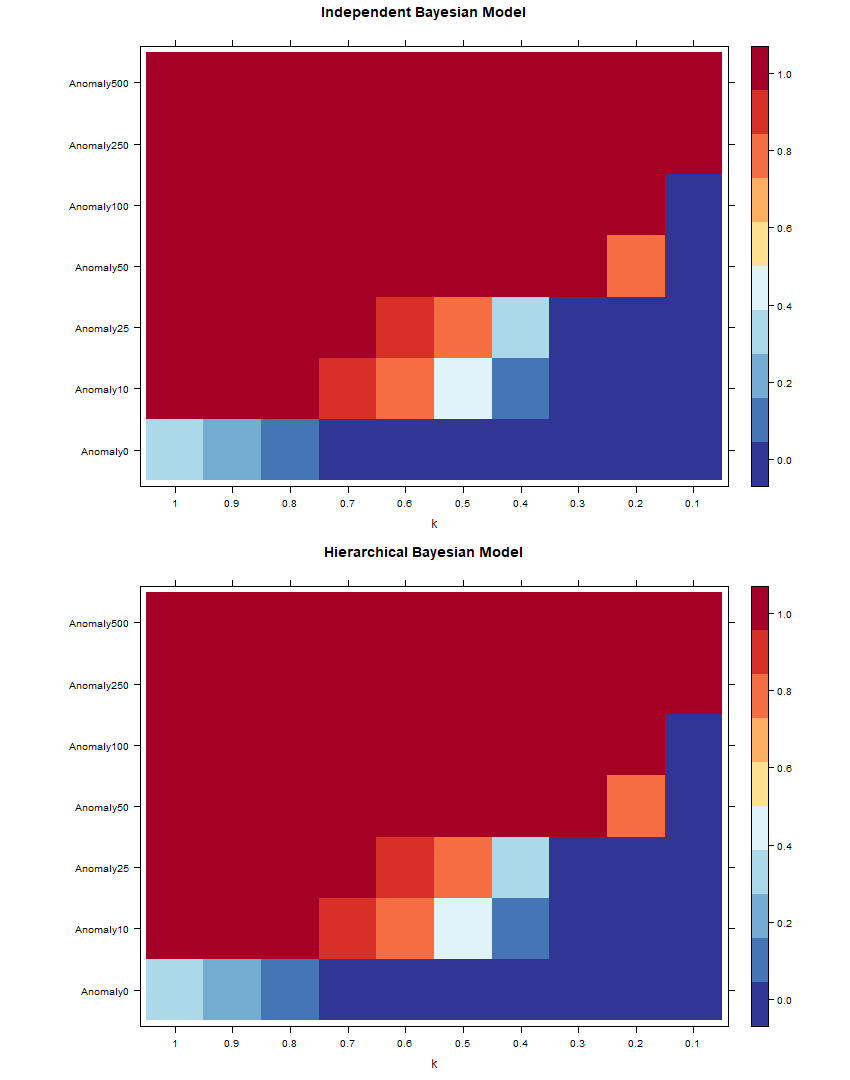
\includegraphics[width=1\linewidth]{../../R-codes/JAGS/plots/sim1/heattotal}
	\caption{Heat-map of anomaly alarms for different size of anomaly under different k values, of IBM and HBM, at category total.}
	\label{fig:heattotalab}
\end{figure}

\newpage

\begin{figure}[!h]
	\centering
	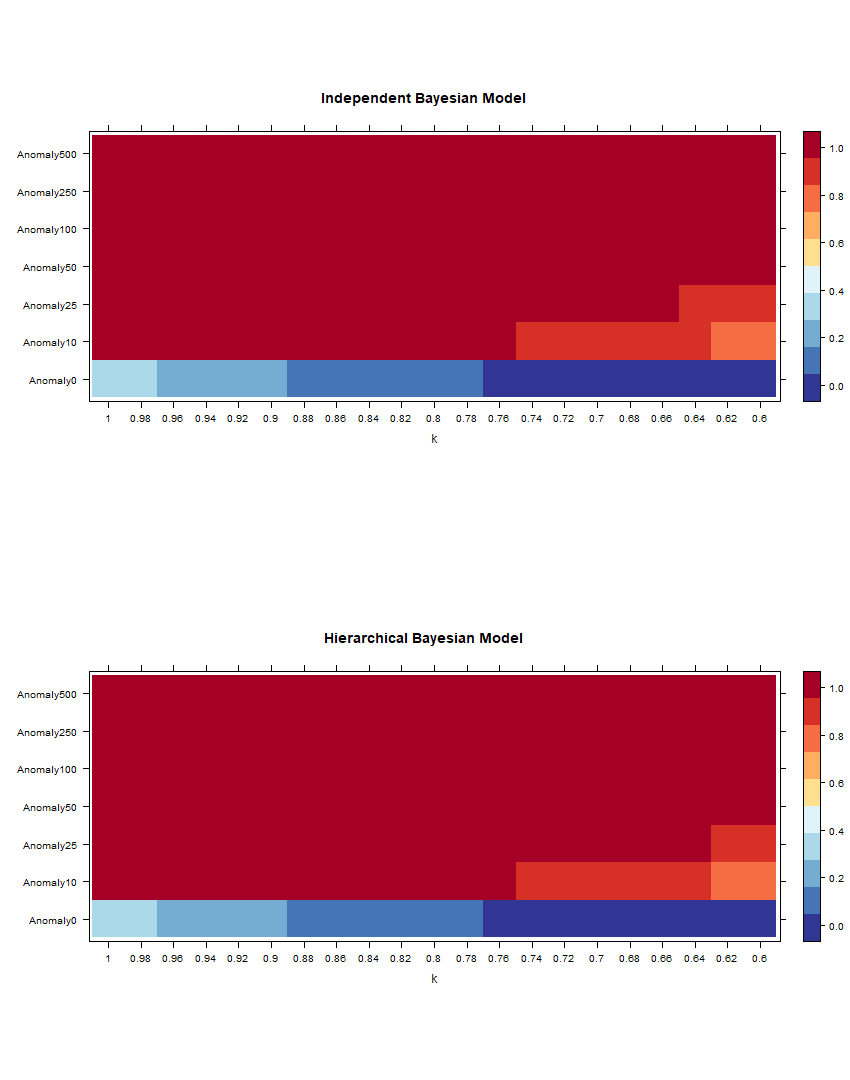
\includegraphics[width=1\linewidth]{../../R-codes/JAGS/plots/sim1/heattotal2}
	\caption{Heat-map of anomaly alarms for different size of anomaly under different k values, of IBM and HBM zoomed in at k values of 0.6 to 1, at category total.}
	\label{fig:heattotalab2}
\end{figure}

\newpage

The heat-map in figure~\ref{fig:heattotalab} presents the anomaly signals of category total for different increments of anomaly added, with IBM and HBM, against different increments of $k$. Strong anomaly signals (in red) tend to appear toward the top left corner of our heap-map, this indicated that signals of anomaly tend to increase in strength with greater anomaly and higher capacity $k$. Zooming in at looking at $k$ values from 0.6 to 1 in figure~\ref{fig:heattotalab2}, we observe a minimal difference in anomaly detection rate between IBM and HBM for category total. Our observation suggests that the difference between anomaly detection rate is small or close to none for IBM and HBM, on the top level of the hierarchy, for all sizes of the anomaly, in a simulated setting with each category generated independently. 

%-----------------------------------------------------------------------------------------
\newpage

\begin{figure}[!h]
	\centering
	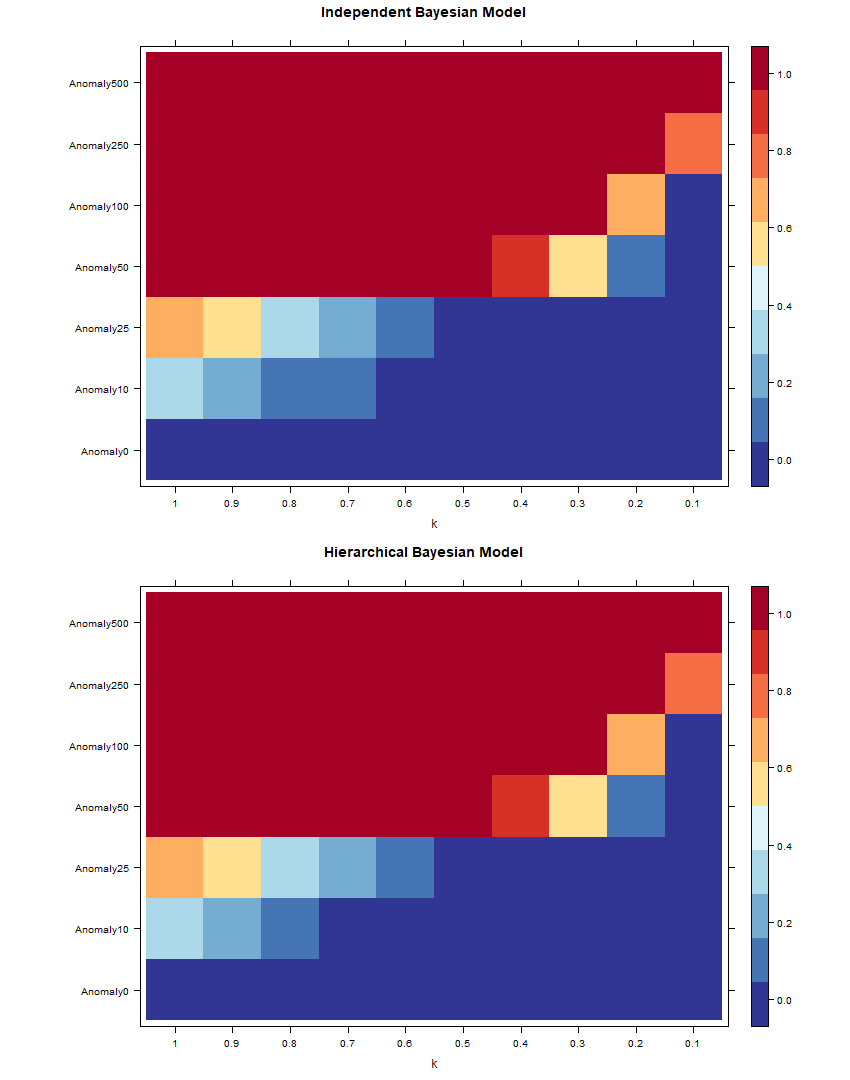
\includegraphics[width=1\linewidth]{../../R-codes/JAGS/plots/sim1/heatA}
	\caption{Heat-map of anomaly alarms for different size of anomaly under different k values, of IBM and HBM, at category A.}
	\label{fig:heatAab}
\end{figure}

\newpage

\begin{figure}[!h]
	\centering
	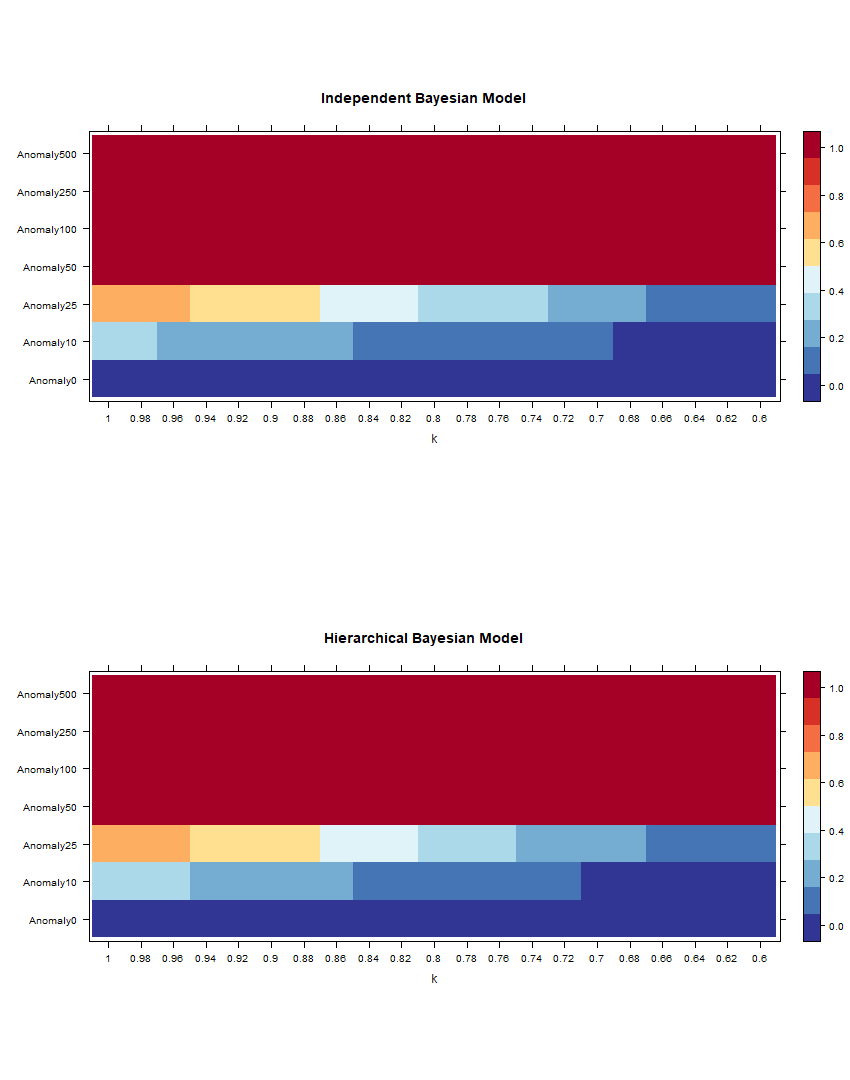
\includegraphics[width=1\linewidth]{../../R-codes/JAGS/plots/sim1/heatA2}
	\caption{Heat-map of anomaly alarms for different size of anomaly under different k values, of IBM and HBM zoomed in at k values of 0.6 to 1, at category A.}
	\label{fig:heatA2ab}
\end{figure}

\newpage

The heat-map in figure~\ref{fig:heatAab} presents the anomaly signals of category A for different increments of anomaly added, with IBM and HBM, against different increments of $k$. Strong anomaly signals (in red) tend to appear toward the top left corner of our heap-map, this indicated that signals of anomaly tend to increase in strength with greater anomaly and higher capacity $k$.Zooming in at looking at k values from 0.6 to 1 in figure~\ref{fig:heatA2ab}, we observe a minimal difference in anomaly detection rate between IBM and HBM for category A. Our observation suggests that the difference between anomaly detection rate is small or close to none for IBM and HBM, on level 2 of the hierarchy, for all sizes of anomaly, in a simulated setting with each category generated independently. 

%-----------------------------------------------------------------------------------------

\newpage

\begin{figure}[!h]
	\centering
	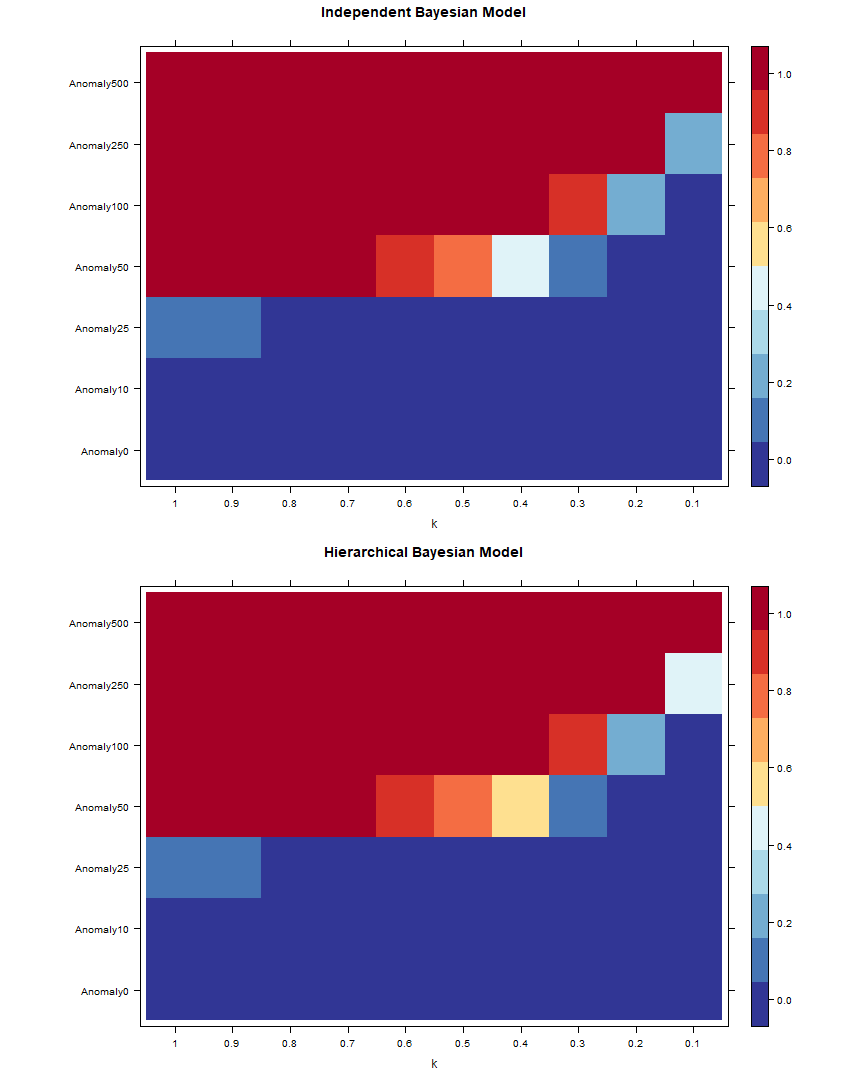
\includegraphics[width=1\linewidth]{../../R-codes/JAGS/plots/sim1/heatAA}
	\caption{Heat-map of anomaly alarms for different size of anomaly under different k values, of IBM and HBM, at category AA.}
	\label{fig:heatAAab}
\end{figure}

\newpage

\begin{figure}[!h]
	\centering
	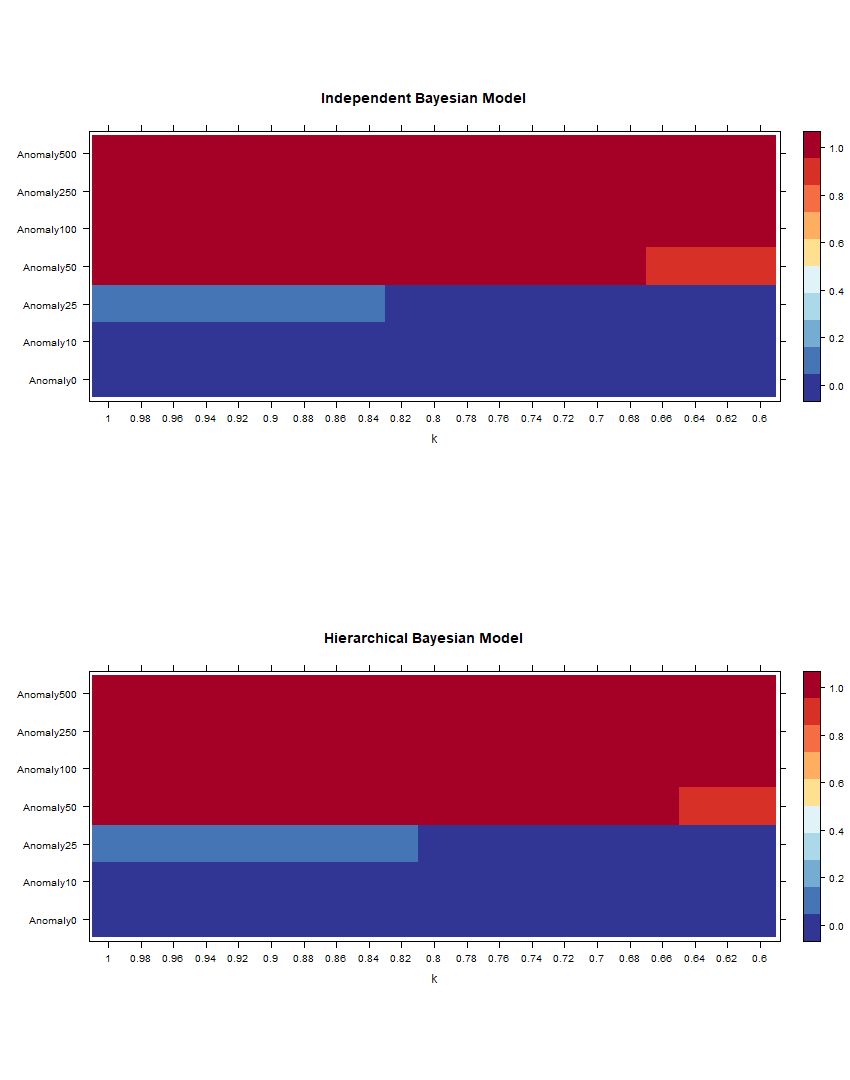
\includegraphics[width=1\linewidth]{../../R-codes/JAGS/plots/sim1/heatAA2}
	\caption{Heat-map of anomaly alarms for different size of anomaly under different k values, of IBM and HBM zoomed in at k values of 0.6 to 1, at category AA.}
	\label{fig:heatAA2ab}
\end{figure}

\newpage
The heat-map in figure~\ref{fig:heatAAab} presents the anomaly signals of category AA for different increments of anomaly added, with IBM and HBM, against different increments of $k$. Strong anomaly signals (in red) tend to appear toward the top left corner of our heap-map, this indicated that signals of anomaly tend to increase in strength with greater anomaly and greater capacity $k$. Zooming in at looking at k values from 0.6 to 1 in figure~\ref{fig:heatAA2ab}, we observe a minimal difference in anomaly detection rate between IBM and HBM for category AA. Our observation suggests that the difference between anomaly detection rate is small or close to none for IBM and HBM, on the bottom of the hierarchy, for all sizes of the anomaly, in a simulated setting with each category generated independently. 

\newpara

Comparing between levels of hierarchies, we observe that for all levels of hierarchy, strong anomaly signals (in red) tend to appear toward the top left corner of our heap-map, confirming the fact that signals of anomaly tend to increase in strength with greater anomaly and higher capacity $k$, for all levels of hierarchy. For all levels of hierarchy, We observe powerful red signals for scenarios with 50\% and more anomalies added, and very weak signals for the case of no anomaly, 10\% anomaly and 25\% anomaly. The overall signals for higher hierarchies tend to be stronger than overall signals in lower hierarchies. 


\subsection{Discussion}

Our DIC results suggest that compared to IBM, HBM gives better goodness of fit and is the better model, for scenarios with different increments of anomalies added to a category at the bottom level of the hierarchy, this provided more evidence that suggests that HBM are superior compared to IBM. Although our DIC comparisons result varies every time we re-ran our JAGS models, the observation appears most of the time, and we have some evidence to back our claim. The finding is consistent with the finds in  \citet{gelman2006multilevel}, that hierarchical models tend to give a better prediction compare to no-pooling (independent) models in all levels. Although our DIC result suggests that HBM gives a different and better posterior distribution, it is kind of hard to tell the differences between posterior distributions for IBM and HBM with all the noise present, and this reduced out confidence to our claim. To rule out the noise from uncertainties in Bayesian posterior is a complex and calculation-intensive process and are out of our scope.

\newpara

As the size of the anomaly increases, the number of ESS tend to decrease. The observation is due to the fact that a more substantial increase in anomaly results in a more substantial, more influential constant change in observed values, that produces a strong autocorrelation relationship and this will reduce the independence of the values, this is also the reason why the standard deviation of posterior also tend to increase as we increase the size of anomalies. The reasoning also applies to hierarchical levels, due to the aggregation constraint values at each level tend to increase, and sample distributions tend to approximate towards normal. So when we are dealing with hierarchical datasets, we must take into account the hierarchical structure, there are significant statistical information within the hierarchy and disregarding the hierarchical structure would significantly reduce the power of our models. A tell-tale sign that IBM had disregarded information about the hierarchical structure is that posterior distributions of IBM tend to have a greater ESS compare to HBM, information between levels often translate into correlations, and without this information, the posterior results in each category would be more independent have a greater ESS. The loss of information becomes more apparent for lower levels of hierarchy; this is because values of a category at a lower level of hierarchy often influenced by an increasing number of more population-level parameter. 

\newpara

With our posterior distributions, we were able to set up a theoretical threshold and made attempts to detect anomalies. Signals of anomaly tend to increase in strength with larger anomalies and higher capacity ($k$), for all levels of hierarchy. Our observations made sense; it is easier to detect larger anomalies because the posterior will be larger and more likely to fall over the threshold. Also, as capacity increase, the average expected value closer to the threshold, and it becomes easier a higher than expected value to go over the threshold. I.e. for a capacity of 80\%, we need a positive anomaly 1.25 times the expected value to meet the threshold, for a capacity of 40\%, we need a positive anomaly 2.5 times the expected value to meet the threshold. Relating to the idea of congestion mentioned in the previous section,  for a hospital to decrease the likelihood of encountering congestion, we would need to decrease the operation capacity of its facilities. Operating at a high capacity may save resource, but is the downside worth it? Did the policymaker take in an account of adverse effects such as doctors getting burnout and an increasing likelihood of congestion, and does the risk out weight the benefit? 

\newpage

\section{Simulation 3: Structure }

\subsection{Simulation setups }

In section 2.5, we present the results of the posterior distribution calculations for the synthesised data, with same 10\% anomaly added on category AA on level 2 (leaf) of the hierarchy, but for hierarchies with a different structure. Most of the hierarchical structure is controlled to be the same, except for the branching at category A. We create 12 scenarios with category A branching into 1 to 12 subgroups equal in size. So for branch = 1,  category A will branch into one subcategory AA, category AA will contain 100\% of the size of the category. For branch = 3, category A will branch into three subcategory AA, AB and AC, category AA, AB and AC will each contain 33\% of the size of category A. 

\subsection{Results}

\begin{table}[ht]
	\centering
	\begin{tabular}{rrrrrrr}
		\hline
		Branch & Min. & 1st Qu. & Median & Mean & 3rd Qu. & Max. \\ 
		\hline
		1 & -7.033 & -1.960 & -0.809 & -1.527 & 0.294 & 1.172 \\ 
		2 & -4.435 & -2.722 & -0.994 & -0.591 & 0.214 & 6.308 \\ 
		3 & -2.710 & -1.013 & 0.554 & 0.521 & 1.440 & 4.575 \\ 
		4 & -3.418 & -0.451 & 0.370 & 0.305 & 1.422 & 3.356 \\ 
		5 & -2.715 & -1.447 & -1.065 & -0.318 & 1.022 & 2.791 \\ 
		6 & -3.082 & -0.733 & -0.129 & 0.121 & 1.042 & 4.216 \\ 
		7 & -4.280 & -2.843 & -1.286 & -1.581 & -0.213 & 0.790 \\ 
		8 & -4.349 & -2.215 & -0.967 & -0.422 & 1.065 & 7.971 \\ 
		9 & -4.931 & -1.649 & -0.335 & -0.303 & 1.014 & 4.038 \\ 
		10 & -5.247 & -1.578 & -0.234 & -0.668 & 0.618 & 3.247 \\ 
		11 & -2.597 & -1.126 & 1.002 & 0.466 & 1.655 & 3.751 \\ 
		12 & -3.340 & -1.786 & -0.102 & 0.223 & 1.838 & 4.623 \\ 
		\hline
	\end{tabular}
	\caption{DIC comparisons for branching number at A} 
	\label{tab:dicanomaly2}
\end{table}

Table~\ref{tab:dicanomaly2} gives the comparison of DIC distributions of Independent Bayesian Model (IBM) and Hierarchical Bayesian Model (HBM) for scenarios with a different hierarchical structure. For all scenarios, the mean and median value is mostly negative; the negative signals suggest that HBM seem to perform better than IBM, most of the time. Uncertainty in Bayesian estimations still exist and have impacts on the reliability of our DIC comparison, although we mostly see negative values for median and mean of the DIC difference distribution, the signal still shifts every time our JAGS model is re-run. Our observation suggests that although there might be a difference between IBM and HBM, it might not be a very big difference. 

\newpage 

\begin{table}[!t]
	\centering
	\begin{tabular}{rrrrrrrr}
		\hline
		Branch & mean & sd & 2.5\% & 50\% & 97.5\% & Rhat & n.eff \\ 
		\hline
		1 & 21.2367 & 4.7008 & 12.9239 & 20.9013 & 31.1209 & 1 & 2787 \\ 
		2 & 21.4198 & 4.6439 & 13.5516 & 20.9515 & 31.6895 & 1 & 2904 \\ 
		3 & 30.4154 & 5.6673 & 20.1950 & 30.2022 & 42.1275 & 1 & 2877 \\ 
		4 & 13.1540 & 3.5731 & 6.9948 & 12.7660 & 21.1359 & 1 & 3000 \\ 
		5 & 26.4296 & 5.0584 & 17.2806 & 26.1034 & 37.3137 & 1 & 2815 \\ 
		6 & 22.3157 & 4.7457 & 14.0816 & 22.0346 & 32.1219 & 1 & 2881 \\ 
		7 & 17.2269 & 4.1264 & 10.2189 & 16.7961 & 26.4545 & 1 & 2587 \\ 
		8 & 19.1497 & 4.3697 & 11.4783 & 18.8391 & 28.4958 & 1 & 3000\\ 
		9 & 27.4028 & 5.2818 & 18.0539 & 26.9926 & 38.6413 & 1 & 2854 \\ 
		10 & 18.2805 & 4.2982 & 10.6334 & 18.0157 & 27.3239 & 1 & 3028 \\ 
		11 & 22.2082 & 4.7100 & 13.9406 & 21.8632 & 32.7639 & 1 & 3000 \\ 
		12 & 23.2141 & 4.8762 & 14.6652 & 22.8895 & 33.4077 & 1 & 3090 \\ 
		\hline
	\end{tabular}
	\caption{Posterior distributions of different models for Total, with different brnch number at A, and calculated with Independent Bayes model} 
	\label{tab:pstprototal}
\end{table}

\begin{table}[!h]
	\centering
	\begin{tabular}{rrrrrrrr}
		\hline
		Branch & mean & sd & 2.5\% & 50\% & 97.5\% & Rhat & n.eff \\ 
		\hline
		1 & 21.1342 & 4.6356 & 13.0372 & 20.8723 & 31.0156 & 1 & 2899 \\ 
		2 & 21.4399 & 4.6658 & 13.3765 & 21.0743 & 31.3564 & 1 & 2888 \\ 
		3 & 30.4796 & 5.5918 & 20.4537 & 30.1087 & 42.6573 & 1 & 3069 \\ 
		4 & 13.0428 & 3.6218 & 6.9370 & 12.7050 & 21.1728 & 1 & 2798 \\ 
		5 & 26.4792 & 5.0783 & 17.5450 & 26.1769 & 37.5123 & 1 & 2903 \\ 
		6 & 22.5513 & 4.7242 & 14.3816 & 22.2968 & 32.5958 & 1 & 3000 \\ 
		7 & 17.2175 & 4.1172 & 9.9473 & 16.9176 & 25.9870 & 1 & 3000 \\ 
		8 & 19.2860 & 4.3666 & 11.7869 & 19.0001 & 28.9699 & 1 & 2712 \\ 
		9 & 27.4363 & 5.2930 & 18.1801 & 27.1123 & 38.8600 & 1 & 2719 \\ 
		10 & 18.3153 & 4.2436 & 10.9404 & 18.0915 & 27.1782 & 1 & 2961 \\ 
		11 & 22.2699 & 4.7638 & 13.7242 & 21.8257 & 32.6838 & 1 & 3000 \\ 
		12 & 23.3112 & 4.9101 & 14.5832 & 22.9914 & 33.6660 & 1 & 3006 \\ 
		\hline
	\end{tabular}
	\caption{Posterior distributions of different models for Total, with different branch number at A, and calculated with Hierarchical Bayes model} 
	\label{tab:pstprototalh}
\end{table}

Table~\ref{tab:pstprototal} and table~\ref{tab:pstprototalh} gives the posterior distribution of the category total, for scenarios with different hierarchical structure. Our results show a large variability between posterior distribution for category total at the top of the structure hierarchy, but there are no obvious trends for different hierarchical structures and IBM and HBM models in any of the values due to the presence of noise. 

\newpage

\begin{table}[!t]
	\centering
	\begin{tabular}{rrrrrrrr}
		\hline
		Branch & mean & sd & 2.5\% & 50\% & 97.5\% & Rhat & n.eff \\ 
		\hline
		1 & 10.2222 & 3.2257 & 4.9491 & 9.9313 & 17.3630 & 1 & 3000 \\ 
		2 & 7.2101 & 2.5820 & 3.0653 & 6.9089 & 13.0457 & 1& 3135 \\ 
		3 & 13.3965 & 3.5903 & 7.1940 & 13.0422 & 21.4547 & 1 & 2843 \\ 
		4 & 5.2344 & 2.2966 & 1.7544 & 4.9212 & 10.8095 & 1 & 2659 \\ 
		5 & 12.2653 & 3.5442 & 6.3801 & 11.9468 & 20.0809 & 1 & 2831 \\ 
		6 & 12.4534 & 3.5617 & 6.4566 & 12.0511 & 20.3078 & 1 & 2826 \\ 
		7 & 11.3345 & 3.3140 & 5.6904 & 11.0780 & 18.6164 & 1 & 2763 \\ 
		8 & 11.3301 & 3.4455 & 5.6405 & 10.9504 & 18.8542 & 1 & 3000 \\ 
		9 & 15.2998 & 3.9278 & 8.5925 & 15.0144 & 24.1089 & 1 & 3000\\ 
		10 & 10.2282 & 3.2404 & 4.9712 & 9.8590 & 17.4283 & 1 & 2719 \\ 
		11 & 12.2384 & 3.5230 & 6.2765 & 11.9505 & 19.9642 & 1 & 3000 \\ 
		12 & 16.2605 & 4.1472 & 9.1019 & 15.9211 & 25.5411 & 1 & 2614 \\ 
		\hline
	\end{tabular}
	\caption{Posterior distributions of different models for A , with different branch number at A, and calculated with independent Bayes model} 
	\label{tab:pstproA}
\end{table}

\begin{table}[!h]
	\centering
	\begin{tabular}{rrrrrrrr}
		\hline
		Branch & mean & sd & 2.5\% & 50\% & 97.5\% & Rhat & n.eff \\ 
		\hline
		1 & 10.3658 & 3.2745 & 4.9563 & 9.9946 & 17.5591 & 1 & 2480 \\ 
		2 & 7.1699 & 2.7092 & 2.8318 & 6.7969 & 13.3853 & 1 & 2763 \\ 
		3 & 13.5106 & 3.6263 & 7.2349 & 13.2756 & 21.5433 & 1 & 2721 \\ 
		4 & 4.9821 & 2.1601 & 1.7617 & 4.6571 & 9.9815 & 1 & 2848 \\ 
		5 & 12.2966 & 3.5260 & 6.2470 & 11.9827 & 20.1420 & 1 & 2691 \\ 
		6 & 11.9993 & 3.3669 & 6.1917 & 11.7362 & 19.3448 & 1 & 2515 \\ 
		7 & 11.1468 & 3.3194 & 5.5362 & 10.8140 & 18.2800 & 1 & 2791 \\ 
		8 & 10.9205 & 3.2059 & 5.5478 & 10.6286 & 17.9246 & 1 & 2596 \\ 
		9 & 15.1743 & 3.7615 & 8.6417 & 14.8581 & 23.3316 & 1 & 2371 \\ 
		10 & 9.4961 & 2.9241 & 4.6206 & 9.1667 & 16.0461 & 1 & 2730 \\ 
		11 & 11.7279 & 3.3009 & 5.9251 & 11.4201 & 18.8472 & 1 & 2389 \\ 
		12 & 15.4642 & 3.7186 & 9.0081 & 15.1212 & 23.5432 & 1 & 2361 \\ 
		\hline
	\end{tabular}
	\caption{Posterior distributions of different modelsfor A , with different branch number at A, and calculated with Hierarchical Bayes model} 
	\label{tab:pstproAh}
\end{table}

Table~\ref{tab:pstprototal} and table~\ref{tab:pstprototalh} gives the posterior distribution of the category A, for scenarios with different hierarchical structure. Our results show a large variability between posterior distribution for category total at the top of the structure hierarchy, but there are no obvious trends for different hierarchical structures and IBM and HBM models in any of the values due to the presence of noise. 

\newpage

\begin{table}[!t]
	\centering
	\begin{tabular}{rrrrrrrr}
		\hline
		Branch & mean & sd & 2.5\% & 50\% & 97.5\% & Rhat & n.eff \\ 
		\hline
		1 & 10.3390 & 3.3313 & 4.9841 & 9.9711 & 18.0423 & 1 & 3015 \\ 
		2 & 2.2864 & 1.4796 & 0.4436 & 1.9694 & 5.9125 & 1 & 2383 \\ 
		3 & 4.3819 & 2.1286 & 1.2499 & 4.0705 & 9.5828 & 1 & 2021 \\ 
		4 & 2.2971 & 1.5500 & 0.3511 & 1.9390 & 6.0469 & 1 & 1776 \\ 
		5 & 4.3729 & 2.0611 & 1.2799 & 4.0873 & 9.4255 & 1 & 1568 \\ 
		6 & 5.1595 & 2.0347 & 1.8054 & 4.9425 & 9.5605 & 1 & 1448 \\ 
		7 & 3.2759 & 1.6852 & 0.7437 & 3.0322 & 7.3844 & 1 & 1259 \\ 
		8 & 3.2901 & 1.6666 & 0.7674 & 3.0726 & 7.0195 & 1 & 1255 \\ 
		9 & 3.1983 & 1.5386 & 0.8286 & 3.0263 & 6.7680 & 1 & 1424 \\ 
		10 & 4.3662 & 1.5571 & 1.6687 & 4.1853 & 7.6161 & 1 & 1110 \\ 
		11 & 2.1852 & 1.3714 & 0.2855 & 1.9361 & 5.4025 & 1 & 1077 \\ 
		12 & 2.9119 & 1.4034 & 0.7174 & 2.6996 & 6.1571 & 1 & 947 \\ 
		\hline
	\end{tabular}
	\caption{Posterior distributions of different models for AA, with different branch number at A, and calculated with independent Bayes model} 
	\label{tab:pstproAA}
\end{table}

\begin{table}[!h]
	\centering
	\begin{tabular}{rrrrrrrr}
		\hline
		Branch & mean & sd & 2.5\% & 50\% & 97.5\% & Rhat & n.eff \\ 
		\hline
		1 & 10.3563 & 3.2788 & 4.9509 & 10.0156 & 17.7970 & 1 & 2540 \\ 
		2 & 2.1951 & 1.5255 & 0.3203 & 1.8362 & 5.9132 & 1 & 1978 \\ 
		3 & 4.5592 & 2.2061 & 1.2605 & 4.2379 & 9.5741 & 1 & 1910 \\ 
		4 & 2.2663 & 1.5396 & 0.3203 & 1.9350 & 5.9029 & 1 & 1540 \\ 
		5 & 4.4613 & 1.9943 & 1.3097 & 4.2350 & 8.8343 & 1 & 1354 \\ 
		6 & 5.2129 & 2.0225 & 1.8571 & 5.0210 & 9.6588 & 1 & 1023 \\ 
		7 & 3.3193 & 1.6606 & 0.7695 & 3.0899 & 7.1315 & 1 & 1053 \\ 
		8 & 3.3147 & 1.6493 & 0.7960 & 3.0817 & 7.1798 & 1 & 1023 \\ 
		9 & 3.2724 & 1.6032 & 0.7633 & 3.0402 & 6.8838 & 1 & 711 \\ 
		10 & 4.4763 & 1.6416 & 1.7625 & 4.3287 & 8.0546 & 1 & 737\\ 
		11 & 2.2327 & 1.2427 & 0.3545 & 2.0587 & 4.9807 & 1 & 952 \\ 
		12 & 3.0880 & 1.4240 & 0.8039 & 2.9188 & 6.2747 & 1 & 816 \\ 
		\hline
	\end{tabular}
	\caption{Posterior distributions of different modelsfor AA, with different branch number at A, and calculated with Hierarchiacl Bayes model} 
	\label{tab:pstproAAh}
\end{table}

Table~\ref{tab:pstproAA} and table~\ref{tab:pstproAAh} gives the posterior distribution of category A, for scenarios with a different hierarchical structure. Our results show a large variability between posterior distribution for category total at the top of the structure hierarchy, unlike what we observe in previous tables, the trend in the number of branch and differences between IBM and HBM is now much more apparent.  Increasing the size of branch at category A decreases mean standard deviation and ESS. Also, posterior mean results for HBM is slightly larger compared to mean results for IBM. 
		
		\begin{figure}[!h]
			\centering
			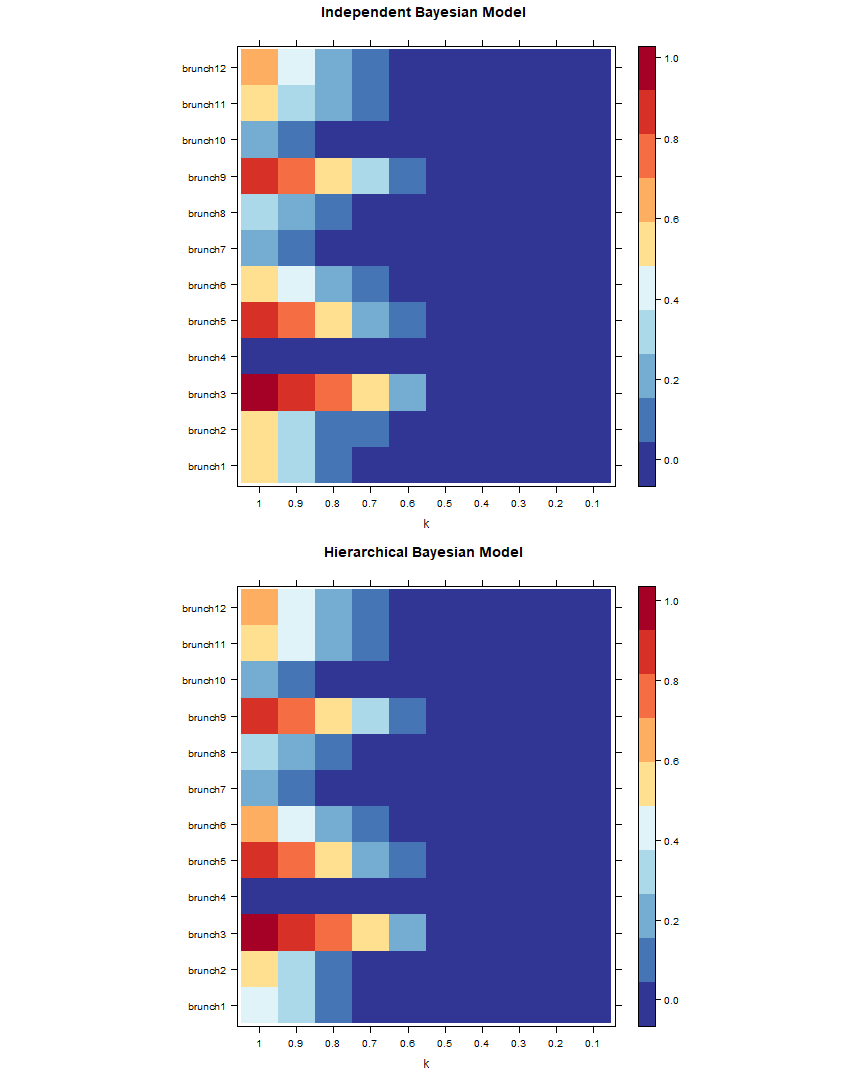
\includegraphics[width=1\linewidth]{../../R-codes/JAGS/plots/sim2/heattotal}
			\caption{Heat-map of anomaly signals for different different hierarchical structure, of IBM and HBM at category total.}
			\label{fig:heattotal3}
		\end{figure}
		
		\newpage
		
		\begin{figure}[!h]
			\centering
			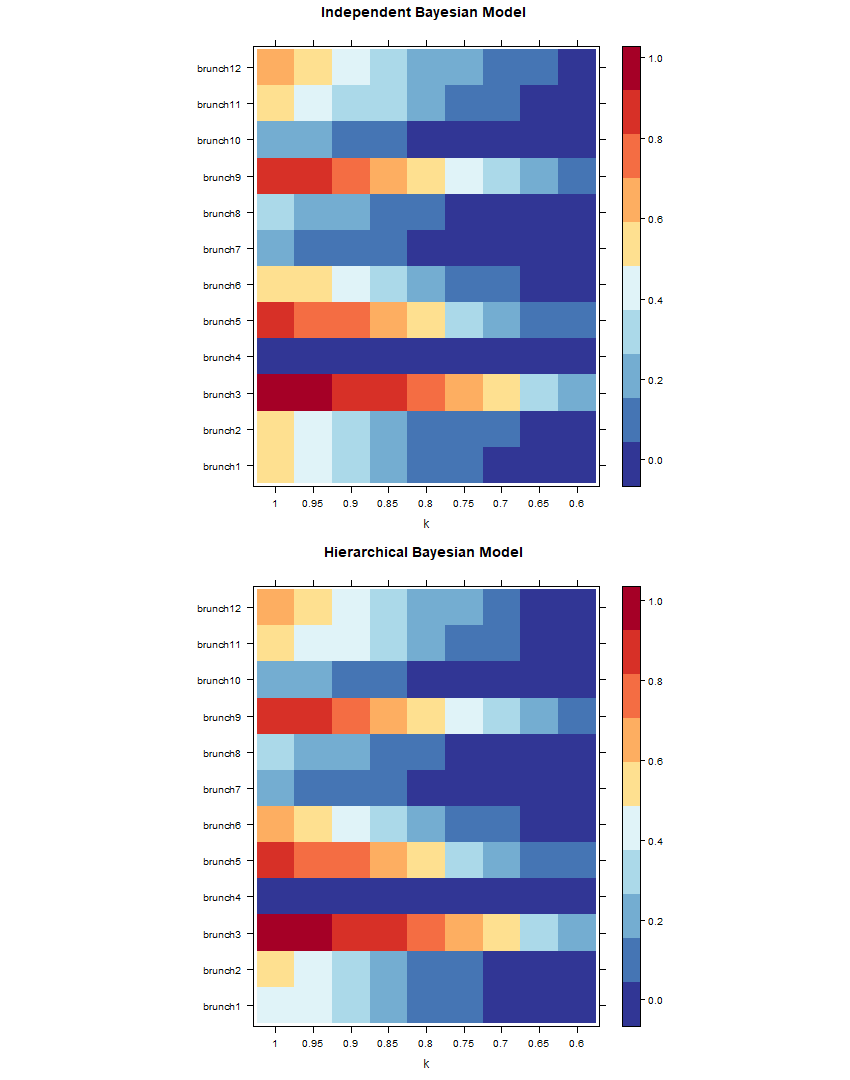
\includegraphics[width=1\linewidth]{../../R-codes/JAGS/plots/sim2/heattotal2}
			\caption{Heat-map of anomaly signals for different different hierarchical structure, of IBM and HBM zoomed in at k values of 0.6 to 1, at category total.}
			\label{fig:heattotal3h}
		\end{figure}
		
		\newpage
		
		The heat-map in figure~\ref{fig:heattotal3} presents the anomaly signals of category total for different hierarchical structures with the addition of a constant anomaly, with IBM and HBM, against different increments of $k$. There is no apparent trend in anomaly signals terms of the number of branch at category AA, of category total. However,  it is relatively clear that stronger signals of anomaly seem to locate at left sider of the heat-map, indicating that higher the $k$, stronger the signal. Zooming in at looking at k values from 0.6 to 1 in figure~\ref{fig:heattotal3h}, we observe a noticeable small difference in anomaly detection rate between IBM and HBM for category total. Our observation suggests that the difference between anomaly detection rate is small or close to none for IBM and HBM, on the top level of the hierarchy, for anomaly with a different hierarchical structure, in a simulated setting with each category generated independently. 
		
		\newpage
		
		\begin{figure}[!h]
			\centering
			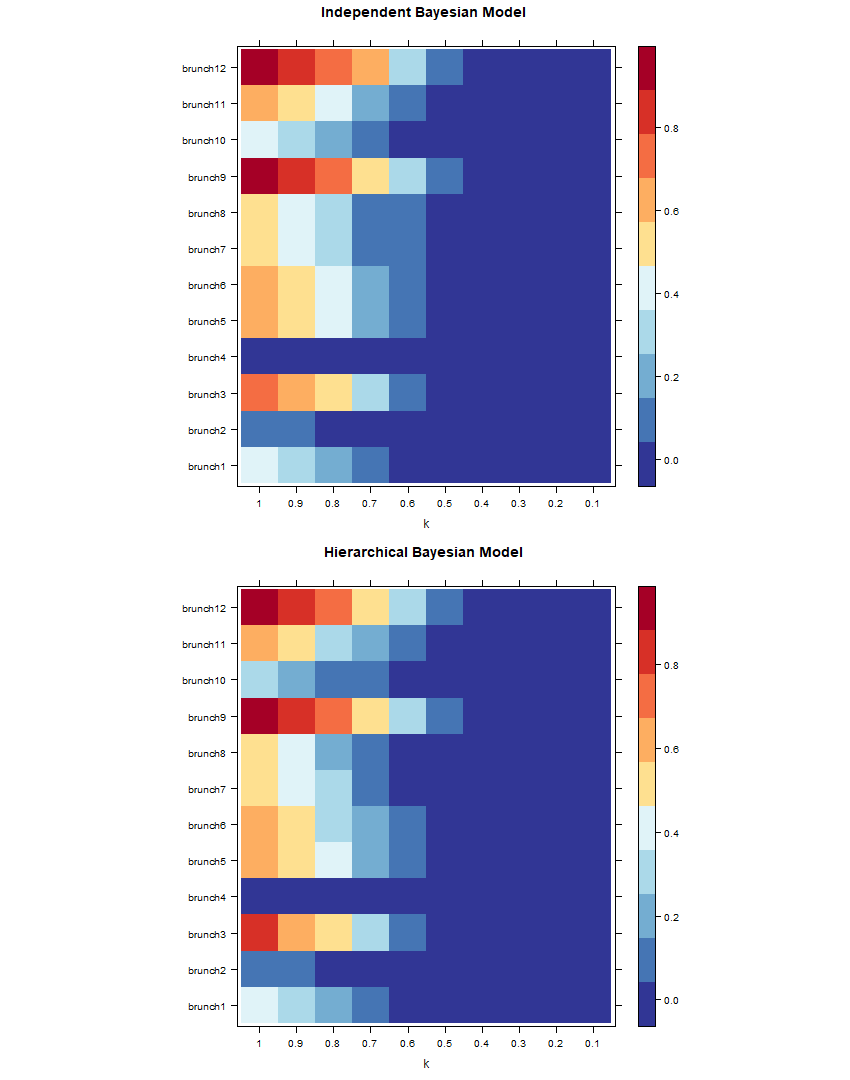
\includegraphics[width=1\linewidth]{../../R-codes/JAGS/plots/sim2/heatA}
			\caption{Heat-map of anomaly signals for different different hierarchical structure, of IBM and HBM, at category A.}
			\label{fig:heatA3}
		\end{figure}
		
		\newpage
		
		\begin{figure}[!h]
			\centering
			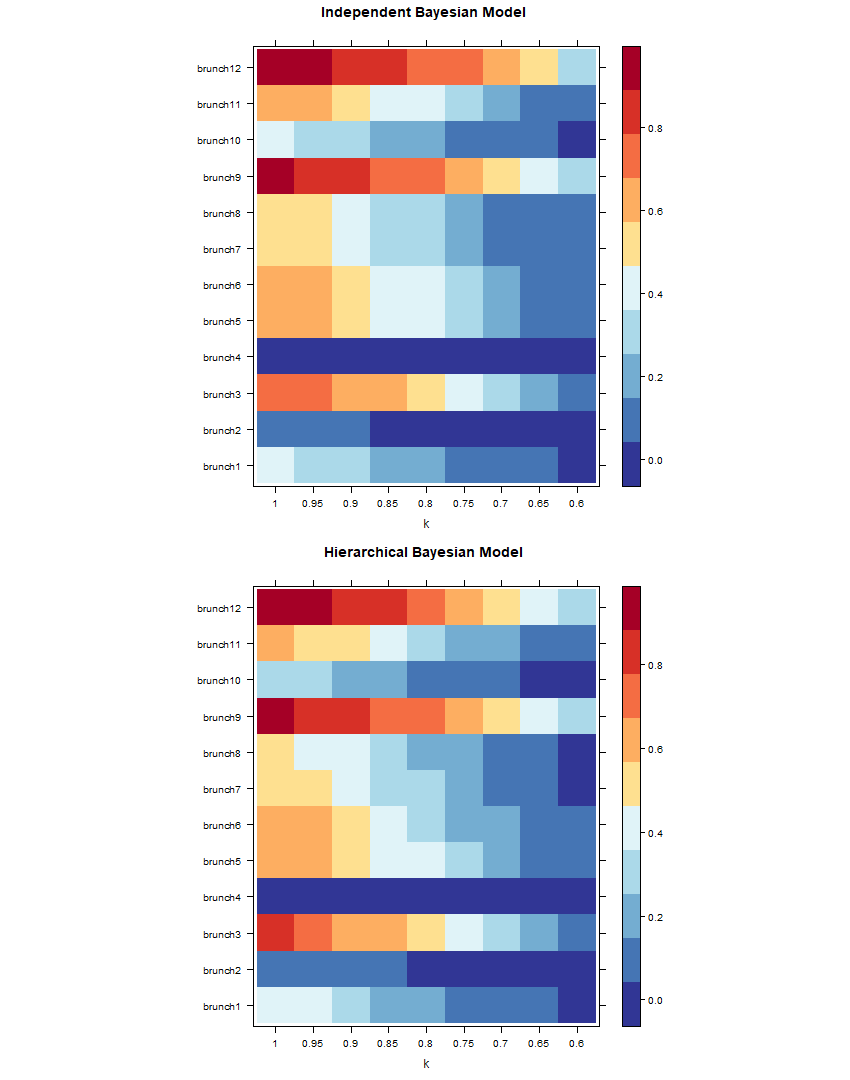
\includegraphics[width=1\linewidth]{../../R-codes/JAGS/plots/sim2/heatA2}
			\caption{Heat-map of anomaly signals for different different hierarchical structure, of IBM and HBM zoomed in at k values of 0.6 to 1, at category A.}
			\label{fig:heatA3h}
		\end{figure}
		
		\newpage
		
		The heat-map in figure~\ref{fig:heatA3} presents the anomaly signals of category A for different hierarchical structures with the addition of a constant anomaly, with IBM and HBM, against different increments of $k$. There is no apparent trend in anomaly signals terms of the number of branch at category AA, of category A. However,  it is relatively clear that stronger signals of anomaly seem to locate at left sider of the heat-map, indicating that higher the $k$, stronger the signal. Zooming in at looking at k values from 0.6 to 1 in figure~\ref{fig:heatA3h}, we observe a noticeable small difference in anomaly detection rate between IBM and HBM for category A. Our observation suggests that the difference between anomaly detection rate is small or close to none for IBM and HBM, on level 2 of the hierarchy, for anomaly with a different hierarchical structure, in a simulated setting with each category generated independently. 
		
		\newpage
		
		\begin{figure}[!h]
			\centering
			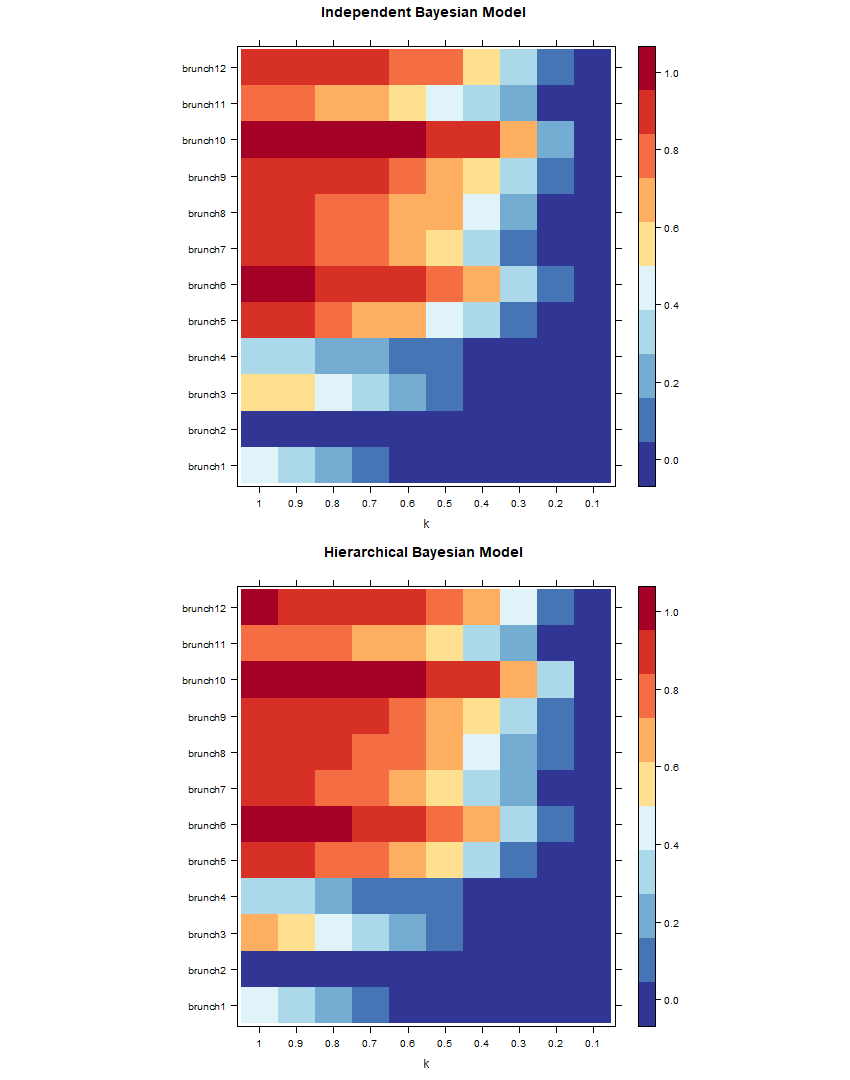
\includegraphics[width=1\linewidth]{../../R-codes/JAGS/plots/sim2/heatAA}
			\caption{Heat-map of anomaly signals for different different hierarchical structure, of IBM and HBM, at category AA.}
			\label{fig:heatAA3}
		\end{figure}
		
		\newpage
		
		\begin{figure}[!h]
			\centering
			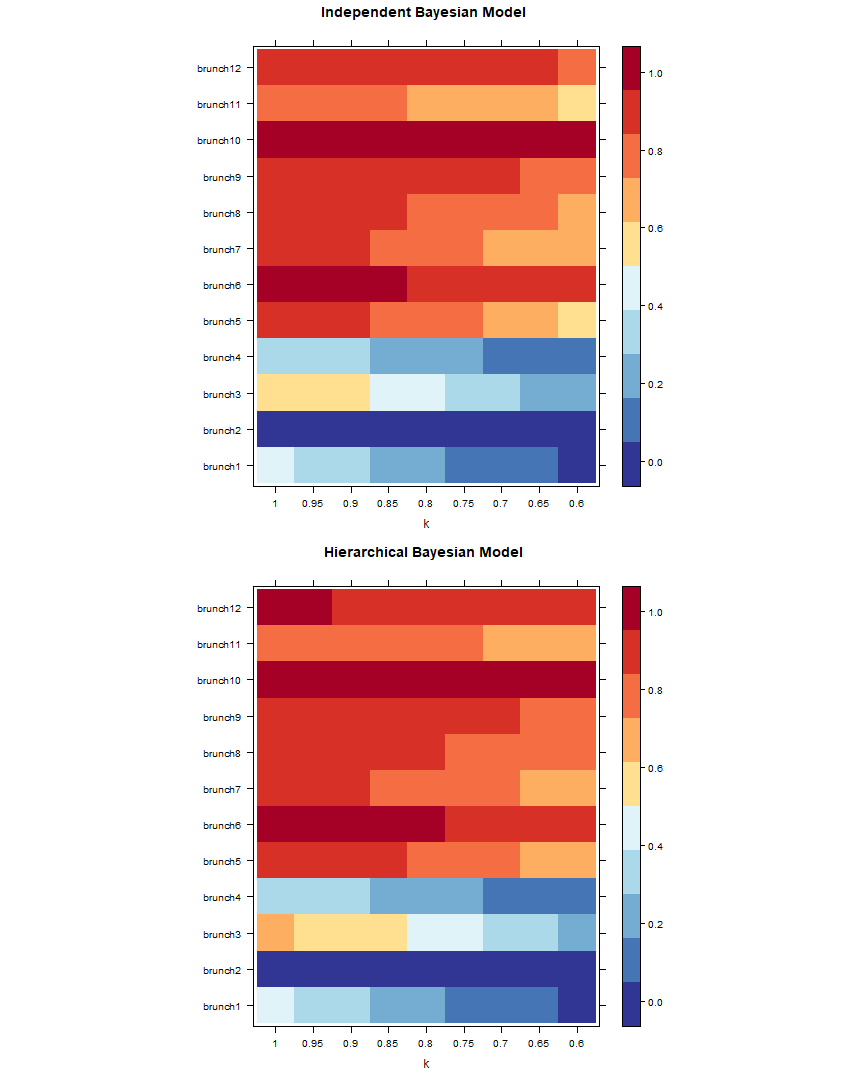
\includegraphics[width=1\linewidth]{../../R-codes/JAGS/plots/sim2/heatAA2}
			\caption{Heat-map of anomaly signals for different different hierarchical structure, of IBM and HBM zoomed in at k values of 0.6 to 1, at category AA.}
			\label{fig:heatAAh3}
		\end{figure}
	
	\newpage
		
		The heat-map in figure~\ref{fig:heatAA3} presents the anomaly signals of category A for different hierarchical structures with the addition of a constant anomaly, with IBM and HBM, against different increments of $k$. Unlike previous categories, anomaly signals tend to get stronger as the number of branching increases. It is also very clear that stronger signals of anomaly seem to locate at left side of the heat-map, indicating that higher the $k$, stronger the signal. Zooming in at looking at k values from 0.6 to 1 in figure~\ref{fig:heatAAh3}, we observe a noticeable small difference in anomaly detection rate between IBM and HBM for category AA. Our observation suggests that the difference between anomaly detection rate is small or close to none for IBM and HBM, on the bottom of the hierarchy, for anomaly with a different hierarchical structure, in a simulated setting with each category generated independently. 
		
		\newpara
		
		Overall we see that there are slight differences in signals fro IBM and HBM results, and if we zoom in and look at a smaller interval of $k$, the difference are more apparent. HBM tend to give strong signals than IBM. Because we simulated datasets used for each scenario independently, there is a lot of uncertainty and noise and made it hard to distinguish differences and trends. However, at the bottom level, where the difference in structure takes place, the effect of noise does not seem to mask the trends any more. Comparing across levels, we see that the top hierarchy have the lowest signal overall, and the bottom hierarchy have the strongest signal overall. 
		
		\subsection{Discussion}
		
		Our DIC results yield similar results as what we have in the previous simulation, that HBM gives better goodness of fit and is the better model, for scenarios with different hierarchical structures. Our finding could suggest that HBM gives better goodness of fit consistently, for hierarchies with different hierarchical structures. These findings add to the reliability of HBM and suggesting it to be a versatile model that is superior to IBM in different settings and for different hierarchical structures. Because we had synthesised datasets used for our scenarios independently, we have a higher level of uncertainty compare to our previous simulation. It adds to the uncertainty we already had from Bayesian estimations and made it even harder to explore for differences and trends. A possible remedy is to use the same dataset, but for branching that take place in category AA, we could try to generate values for its children categories randomly, with statistical techniques such as bootstrapping. 
		
		\newpara
		
		An interesting observation is that trends and differences in category AA seem to have overcome the making effect by the noise and are a lot more clear than what we observe in higher categories. It is partly due to the fact that HBM tend to retain more information ( there is more information at a lower level of hierarchy) at lower levels of hierarchy and the amount of information is significant enough for HBM to produce results that have a stronger presence than randomness. Another possibility is that it has something to do with influences of extra information that we created for Category A and it's children during our data synthesis process, which is retained by HBM but not at all present in IBM. 
		
		
		
